\section{The localized mirror and Morse charts at the nodes}\label{sec:regime}

This section prepares the analytic side of the mirror lift. We fix the members $Y_t$ of Theorem~\ref{thm:main} and
study them near the maximally degenerate limit by comparing monomials in units of $L=\log(1/t)$. Three results are
proved. First, for $t$ small and every coefficient vector in a window around $\mathcal Z$, the member $Y_t$ is smooth
and isotopic in $X_{\mathcal T}$ to a smooth compact submanifold $W^*$, the \emph{localized mirror}, on which every
stratum of the tropical picture near the discriminant has an exact algebraic model (Lemma~\ref{lem:W} and
Proposition~\ref{prop:isotopy}). Second, near the node point (Definition~\ref{def:morsecoords}) of each $P\in Q$ the defining function,
in the trivialisation of the anticanonical bundle by the monomial $\gamma_ax^a$, has exactly one critical point; it is nondegenerate, its critical value differs by $O(t^{\theta_0/2})$ from $-\kappa_P=1-\mu_P^{-1}$,
and on a polydisc around it $W^*$ is exactly the conifold smoothing $\{xy+z_1z_2=\kappa_P\}$ (Lemmas~\ref{lem:NM}
and~\ref{lem:TR}). This defines the vanishing sphere $\delta_q$. Third, a sphere isotopic to $\delta_q$ is the
boundary, over a Lefschetz thimble, of a four-chain $\Pi_q$ lying over a standard half-plane through the node of the
base $B_Y$ of Section~\ref{sec:dualpair}; we orient $\delta_q$ so that this boundary is $\rho_q\,\delta_q$ for every
standard half at $q$ (defined in Section~\ref{ssec:nodepiece}), with either orientation and either sign of its coefficient (Definition~\ref{def:orient} and
Lemma~\ref{lem:SI}). Section~\ref{sec:lift} builds the chains of Theorem~\ref{thm:lift} from these node pieces and from
pieces along the legs of the discriminant.

The localized mirror is modelled on the tropical localizations of Mikhalkin \cite{Mikhalkin} and Yamamoto
\cite[Def.~3.1]{Ya16}: each monomial is multiplied by a cut-off that vanishes where the monomial is far from maximal, so
that near each stratum only the monomials of one cell of the tropical picture survive. Their results assume a unimodular
subdivision; the mirror subdivision contains the node parallelograms and is not unimodular, so their results do not
apply here, and the transport lemma and the isotopy are proved directly. The estimates are comparisons of tropical deficits. The proofs of the one-cell
lemma, of the transport lemma and of the lemmas on the Morse chart are in Appendix~\ref{app:mirror}.

\subsubsection*{Standing assumptions}
In this section and in Sections~\ref{sec:lift} and~\ref{sec:periods} the polytope $\Delta$ is admissible, the profile $\sigma$
satisfies~\ref{hyp:P}, the pair $(\mathcal T,\check h)$ is fixed as in Section~\ref{ssec:tropical}, and $\mathcal F_C$ is
the pulling refinement of $\Sigma'$, with its height $h_C$ (Section~\ref{ssec:mirrorsub}). We use three of the properties
proved in Proposition~\ref{prop:pulling}: $h_C$ induces $\mathcal F_C$, and every maximal cell of the induced subdivision of
$(\partial\Delta\cap N)\cup\{0\}$ contains $0$ (item~(1)); $\mathcal F_C$ agrees with $\Sigma'$ on the two-skeleton, so that its
cells in a two-face of $\Delta$ are the cells of $\sigma$ (Definition~\ref{def:profile}), each without lattice points other
than its vertices (item~(2)); and the \emph{height condition} of item~(4), restated in coordinates in
Definition~\ref{def:node}. The subdivision $\Sigma'$ itself need not satisfy the height condition, which is why the mirror
family is built on $\mathcal F_C$.

\subsubsection*{Constants}
The constants of Sections~\ref{sec:regime} and~\ref{sec:lift} depend on data chosen in a fixed order. First the
\emph{configuration} is fixed: $\Delta$, $\sigma$, $\mathcal T$ and $\check h$, $\mathcal F_C$ and its height $h_C$, the
lattice vectors $w_u$ of Section~\ref{ssec:member}, and the integer $k_0$. A constant is said to \emph{depend only on the
configuration} if it depends on these data alone. Then a compact set $\mathscr C_0\subset\mathcal Z$, a radius $r$ and
a size $\eta_0$ of the perturbation of the node binomials are chosen, then a threshold $t_0$, and finally the
coefficient vector $c$ and $t<t_0$. The principal constants are these.
\begin{center}\small
\begin{tabular}{p{2.4cm}p{7.4cm}p{4.6cm}}
constant & role & fixed in\\\hline
$h_C$ & strictly convex height inducing $\mathcal F_C$ & Section~\ref{ssec:mirrorsub}\\
$k_0$ & multiple of $\varphi$ in the height $H$ & \eqref{eq:lambdagap}, Lemma~\ref{lem:gaps}(4)\\
$\theta_0$ & threshold of the one-cell lemma & Lemma~\ref{lem:onecell}\\
$\mathfrak g_P$, $\mathfrak g_\omega$ & apex gap of a node, vertex gap of a triangle & Definition~\ref{def:node}\\
$\mathcal E_P$, $\mathcal E_{\max}$, $e_{\max}$ & exponent constants & Definition~\ref{def:node}\\
$C_\eta$, $C_{\mathbf R}$ & ratio of the largest to the smallest $|\eta_P|$; bound of $\|\xi\|$ by $\max_P|\eta_P|$ &
Lemma~\ref{lem:eta}; after Definition~\ref{def:window}\\
$\theta_e$ & maximum on the face $E_e$ of the smallest deficit of a monomial other than $0,n,n'$ & Definition~\ref{def:legcell}\\
$\theta_1$, $\theta_2$, $\theta_3$ & cut-off constant; sizes in the torus directions and of the first segments of the
model arcs & Definition~\ref{def:legcell}, Section~\ref{ssec:localized}\\
$\theta_P$ & reach of the node neighbourhood, $\mathfrak g_P/2-\theta_1$ & after~\eqref{eq:lambdagap}\\
$\theta_4$ & size of the germs at the model points & Definition~\ref{def:modelpos}(2)\\
$r_1$, $r$ & radii of the Morse polydisc; $r_1=\min(1/4,(20/C_{\mathbf R})^{1/2})$ & Lemma~\ref{lem:NM}, Definition~\ref{def:window}\\
$\eta_0$ & size of the perturbation of the node binomials, $\eta_0\le r^2/20$ & Definition~\ref{def:window}\\
$\varsigma_{\max}$, $\varsigma_0$ & depth of the pieces & Lemma~\ref{lem:pieces}; Section~\ref{sec:lift}\\
$t_0$ & threshold on $t$, below the threshold $t_1$ of Lemma~\ref{lem:NM} & Lemmas~\ref{lem:W}, \ref{lem:NM}, \ref{lem:TR}
\end{tabular}
\end{center}
These constants exist for every admissible $\Delta$ and every profile satisfying~\ref{hyp:P},
with the conventions below when there are no nodes. The height $h_C$ exists by the regularity of $\mathcal F_C$. The constant
$\theta_0$ is the minimum of finitely many positive values of linear programs (Lemma~\ref{lem:onecell}). The gaps and
the exponent constants are read off from the lattice data, the vectors $w_u$ and the heights, and $k_0$ is any integer
above the explicit bound of Lemma~\ref{lem:gaps}(4), which involves only lattice data and $h_C$. The constants $C_\eta$
and $C_{\mathbf R}$ come from the linear algebra of the vectors $r_P$ (Lemma~\ref{lem:eta}); $\theta_e$, $\theta_1$, $\theta_2$,
$\theta_3$, $\theta_P$ and $r_1$ are explicit; $\theta_4$ and $\varsigma_{\max}$ are bounds over the finitely many
model data of Section~\ref{sec:lift}; and $t_0$ is the minimum of finitely
many thresholds, each given by an explicit inequality in Appendix~\ref{app:mirror}.

\paragraph{The case without nodes.}
When $Q=\emptyset$, we have $K=0$. Put $C_\eta=C_{\mathbf R}=1$ and
$\mathcal E_{\max}=0$, and replace the direction choice of
Lemma~\ref{lem:eta} by $\xi_c=0$, $c=c^{(0)}$.
The window has no binomial-ratio restrictions; the norm bound for $\xi_c$
has empty maximum zero. Omit node-indexed constructions and thresholds,
retaining the triangle-gap, height, edge and trivalent-vertex conditions.
Thus $U_\C$, $U^+_\C$ and $U$ have only their stated bounds on $\|\xi\|$.
Cases~(A) and~(B) in the proof of Lemma~\ref{lem:W} exhaust all points
and use only bounds on coefficient moduli. Compactness of
$\mathscr C_0$ therefore gives a uniform threshold on $t$ for smoothness
of every member of $U^+_\C$. In particular $U^\circ=D_\emptyset=U$.
Theorem~\ref{thm:main}(1)--(2) then follow using zero relations, the zero
cycle and the zero chain, while item~(3) has codimension and relative
Picard number zero. Corollary~\ref{cor:smooth} holds with the trivial
smoothing of the already smooth $X'_\sigma$ and the empty transition of
$Y_t$. All subsequent node calculations concern $Q\ne\emptyset$;
the constructions for non-node tropical pieces remain in force.

\subsection{The mirror member}\label{ssec:member}

\subsubsection*{Toric conventions}
The vertices $u\in\partial\Delta^\circ\cap M$ of $\mathcal T$ span the rays of a complete unimodular fan in $M_\R$, and
$X_{\mathcal T}$ is the corresponding smooth projective toric fourfold, with Cox coordinates $Z_u$ \cite{CLS}. For $n\in\mathcal A=\Delta\cap N$ the Cox monomial
\[
x^n:=\prod_uZ_u^{e_u(n)},\qquad e_u(n):=\langle u,n\rangle+1\ \ge0,
\]
is a section of the anticanonical bundle, and $x^n/x^m=\chi^{n-m}$ is a character of the dense torus $T=M\otimes\C^*$.
The face $u^\vee=\{n\in\Delta:\langle u,n\rangle=-1\}$ of $\Delta$ consists of the lattice points with $e_u(n)=0$; it is
a facet when $u$ is a vertex of $\Delta^\circ$. The origin has $e_u(0)=1$ for every $u$. On the chart
$U_{\mathsf c}\cong\C^4$ of a maximal cone $\mathsf c$ the Cox coordinates $Z_u$, $u\in\mathsf c$, are coordinates and the
others are set to $1$; a point lies on the orbit of a cone $\mathsf c'$ exactly when the $Z_u$ with $u\in\mathsf c'$ vanish
there. We
write $\operatorname{Log}\colon T\to M_\R$ for the map with $\langle\operatorname{Log}x,n\rangle=\log|\chi^n(x)|$. Cells of
$\mathcal F_C$ are denoted $\omega$, as in Section~\ref{sec:dualpair}.

For every edge $[u,u']$ of $\mathcal T$ that lies in a face of $\Delta^\circ$ of dimension at most two we fix an order
$(u,u')$ of its end points and a lattice vector $w_u\in N$ with $\langle u,w_u\rangle=1$ and $\langle u',w_u\rangle=0$
(the fan over $\mathcal T$ is unimodular; for the dual edge of a node, compare Lemma~\ref{lem:primheight}).

\subsubsection*{Heights and the member}
The height is $H=k_0\varphi+h_C$ of Section~\ref{ssec:mirrorfamily}, with $h_C$ as in Section~\ref{ssec:mirrorsub}: strictly
convex on the fan over $\mathcal F_C$, inducing $\mathcal F_C$, with integral slopes and $h_C(0)=0$; and $\varphi$, equal to
$1$ on $\partial\Delta$ and linear on the cones over the faces of $\Delta$, has integral slopes since $\Delta$ is reflexive.
So $H(0)=0$, $H(n)=k_0+h_C(n)$ for $n\in\partial\Delta\cap N$, and $H$ is integral at lattice points; the integer $k_0\ge1$
is fixed below. A subset $I\subseteq\mathcal A$ is \emph{cellular} if the lifted points
$(n,H(n))$, $n\in I$, lie on a common lower face of their convex hull.

\begin{lemma}\label{lem:hull}
For $k_0\ge0$ the lower faces are the polytopes $\operatorname{conv}(0,\omega)$ and $\omega$, $\omega\in\mathcal F_C$, and
their faces. A set $I\subseteq\mathcal A$ is cellular if and only if $I\subseteq\{0\}\cup\omega$ for some cell $\omega$ of
$\mathcal F_C$.
\end{lemma}

\begin{proof}
$H$ is convex, with the cones over the cells of $\mathcal F_C$ as its maximal domains of linearity, since $\varphi$ is
convex and linear on the cones over the faces of $\Delta$ and $h_C$ is strictly convex on the finer fan over
$\mathcal F_C$. The lifted lattice points lie on the graph of $H$, which over $\Delta$ is the lower hull of their convex
hull, because a convex function is at most any convex combination of its values. The domains of linearity of $H$ on
$\Delta$ are the $\operatorname{conv}(0,\omega)$.
\end{proof}

The integer $k_0$ is fixed subject to one lower bound, \eqref{eq:lambdagap} below; by Lemma~\ref{lem:gaps}(4) this
bound holds for every $k_0\ge\max\bigl(2e_{\max},\,6,\,1-\min_{\partial\Delta\cap N}h_C\bigr)$. The
\emph{mirror member} is the member $Y_{t,c}$ of Section~\ref{ssec:mirrorfamily},
\[
Y_t=\{F_t=0\}\subset X_{\mathcal T},\qquad F_t=\sum_{n\in\mathcal A}\gamma_nx^n,\qquad \gamma_n=c_nt^{H(n)},\qquad
0<t<1,
\]
and we put $L:=\log(1/t)$. The coefficient vector $c$ is real with the \emph{sign pattern} $c_0>0$ and $c_n<0$ for
$n\neq0$.

\subsubsection*{Node binomials and the window}
Let $P=abcd$ be a node parallelogram, labelled as in Section~\ref{ssec:admissible}. Since $H$ is linear on the cone over
$P$ and $a+c=b+d$, its node binomial ratio is $\mu_P=c_ac_c/(c_bc_d)=\gamma_a\gamma_c/(\gamma_b\gamma_d)$. The set
$\mathcal Z$ of Section~\ref{ssec:mirrorfamily} is nonempty: it contains the vector with $c_0=1$ and $c_n=-1$ for
$n\neq0$. Fix a compact set $\mathscr C_0\subset\mathcal Z$. As in Section~\ref{ssec:mirrorfamily}, every real $c$ with the
sign pattern is uniquely $c=c^{(0)}e^\xi$ with $c^{(0)}\in\mathcal Z$ and $\xi\in\operatorname{span}_\R\{r_P\}$, and we put
\[
\eta_P:=\log\mu_P=r_P\cdot\xi .
\]

\begin{lemma}\label{lem:eta}
Assume $Q\ne\emptyset$. The map $\xi\mapsto(\eta_P)_P$ has image $V=\{\eta:\sum_Pk_P\eta_P=0$ for every relation $\sum_Pk_Pr_P=0\}$, and no
coordinate $\eta_P$ vanishes identically on $V$. Consequently there are a direction $\bar\xi\in\operatorname{span}\{r_P\}$,
which we fix once for the matrix $\mathbf R$ with rows $r_P$, and a constant $C_\eta\ge1$, depending only on $\mathbf R$ and $\bar\xi$, such that for every $\eta_0>0$ the multiple $\xi$ of
$\bar\xi$ with $\max_P|\eta_P|=\eta_0$ satisfies $\eta_0/C_\eta\le|\eta_P|\le\eta_0$ for all $P$.
\end{lemma}

\begin{proof}
The image is the column space of the matrix $\mathbf R$ with rows $r_P$, which is the annihilator of its left kernel. The
coordinate $\eta_P$ vanishes on it if and only if $e_P$ lies in the left kernel, that is $r_P=0$, which never holds. So
the complement in the image of the hyperplanes $\{\eta_P=0\}$ is dense; take $\bar\xi$ with $\mathbf R\bar\xi$ in it and
$C_\eta=\max_P|r_P\cdot\bar\xi|/\min_P|r_P\cdot\bar\xi|$.
\end{proof}

\begin{definition}[the window]\label{def:window}
Fix $r\in(0,r_1]$, with $r_1$ as in Lemma~\ref{lem:NM}, and $\eta_0\in(0,r^2/20]$. A coefficient vector
$c=c^{(0)}e^{\xi}$ with $c^{(0)}\in\mathscr C_0$ and $\xi\in\operatorname{span}_\R\{r_P\}$ is \emph{in the window} if
$\eta_0/C_\eta\le|\eta_P|\le\eta_0$ for every node. For $c^{(0)}\in\mathscr C_0$ the \emph{complex neighbourhood}
$U_\C=U_\C(c^{(0)})$ is the set of $c^{(0)}e^{\xi}$ with $\xi\in\C^{\mathcal A}$, $\|\xi\|\le1$ and $|\eta_P(\xi)|\le\eta_0$
for every node, and $U^+_\C$ is defined in the same way with the bounds $2$ and $2\eta_0$. Here $\|\xi\|:=\max_n|\xi_n|$,
and $\|\cdot\|_*$ denotes the dual norm, so that $\|r_P\|_*=4$.
\end{definition}

In the notation of Theorem~\ref{thm:main}, $C=C_\eta$ and $\eta_1=r_1^2/20$; for $\eta_0\le\eta_1$ we take $r=r_1$.
Both depend only on the matrix $\mathbf R$ with rows $r_P$ and on the direction $\bar\xi$ of Lemma~\ref{lem:eta}.
Every vector in the window lies in $U_\C$: for $\xi$ in the span of the $r_P$ one has $\|\xi\|\le C_{\mathbf R}\max_P|\eta_P|$,
with $C_{\mathbf R}$ depending only on $\mathbf R$ (the map $\xi\mapsto\mathbf R\xi$ is injective on the span of the rows), and $C_{\mathbf R}\eta_0\le1$, because $\eta_0\le r^2/20\le r_1^2/20$ and
$r_1^2\le20/C_{\mathbf R}$ (Lemma~\ref{lem:NM}). The union of the sets $U^+_\C(c^{(0)})$, $c^{(0)}\in\mathscr C_0$, is compact, so
$|c_n|$ and $|c_n|^{-1}$ are bounded on it by a constant depending on $\mathscr C_0$. Constants called $C$, and the
thresholds on $t$, depend on the configuration and on $\mathscr C_0$ through these bounds, and on $r$ and $\eta_0$ where
this is indicated; we do not repeat the dependence on $\mathscr C_0$. Lemmas~\ref{lem:W}(2), \ref{lem:NM}
and~\ref{lem:TR}(2) are stated for $c\in U^+_\C$, as Section~\ref{sec:periods} requires (Lemma~\ref{lem:U}); their proofs
use only these two-sided bounds on $|c_n|$, the bound $|\eta_P|\le2\eta_0$ and the standing choices $r\le1/4$,
$\eta_0\le r^2/20$. No threshold is uniform on all of
$\mathcal Z$: when $|\log|c^{(0)}_n||$ is comparable to $\theta_0L$ the coefficients move the tropical picture, and the
estimates below fail.

When every singular two-face of $\Delta$ is a unit square, $\mathcal Z$ is the set of real points, with the sign
pattern, of the locus to which Batyrev and Kreuzer specialise the mirror family \cite[\S3]{BK10}, on which the face
polynomial of every square is a product of two binomials. At a hexagon this is different.

\begin{remark}[the face polynomial of a hexagon]\label{rem:hexface}
Let $G$ be a hexagon, in lattice coordinates of its plane with $o=0$ and $w_0,\dots,w_5$ as in
Section~\ref{ssec:admissible}; write its face polynomial as $f_G=c_o+\sum_jc_{w_j}\chi^{w_j}$. The node parallelograms have
their diagonal through $o$, so $\mu_P=c_oc_{w_{j+1}}/(c_{w_j}c_{w_{j+2}})$ for $P=\{o,w_j,w_{j+1},w_{j+2}\}$. The analogues of the
specialisation of \cite{BK10} are the product loci below; we write $\mathsf a_i,\mathsf b_i,\mathsf e_i$ for the
coefficients of the factors.
\begin{enumerate}
\item \emph{$A_1$ branch}, $P_1=\{o,w_0,w_1,w_2\}$, $P_2=\{o,w_3,w_4,w_5\}$ (the other $A_1$ subdivisions are rotations).
For $f_G=(\mathsf a_0+\mathsf a_1\chi^{w_0}+\mathsf a_2\chi^{w_1})(\mathsf b_0+\mathsf b_1\chi^{w_3}+\mathsf b_2\chi^{w_4})$
one finds $c_o=\sum_i\mathsf a_i\mathsf b_i$,
\[
(c_{w_0},\dots,c_{w_5})=(\mathsf a_1\mathsf b_0,\mathsf a_2\mathsf b_0,\mathsf a_2\mathsf b_1,\mathsf a_0\mathsf b_1,\mathsf
a_0\mathsf b_2,\mathsf a_1\mathsf b_2),
\]
and $\mu_{P_1}=\mu_{P_2}=1+(\mathsf a_0\mathsf b_0+\mathsf a_2\mathsf b_2)/(\mathsf a_1\mathsf b_1)$. A real product has real
factors after rescaling (a trinomial whose Newton polygon is a unimodular triangle is irreducible); the sign
conditions $c_{w_j}<0$ then force all $\mathsf a_i$ to have one sign and all $\mathsf b_i$ the other, so
$c_o=\sum_i\mathsf a_i\mathsf b_i<0$: no real point of the product locus has the sign pattern, and in particular none lies
in $\mathcal Z$.
\item \emph{$A_2$ branch}, parallelograms $P_j$, $j\in\{0,2,4\}$ (the odd subdivision is symmetric). For
$f_G=(\mathsf a_0+\mathsf a_1\chi^{w_0})(\mathsf b_0+\mathsf b_1\chi^{w_2})(\mathsf e_0+\mathsf e_1\chi^{w_4})$, since
$w_0+w_2+w_4=0$, $c_o=T_1+T_2$ with $T_1=\mathsf a_0\mathsf b_0\mathsf e_0$, $T_2=\mathsf a_1\mathsf b_1\mathsf e_1$, and
$\mu_{P_j}=1+T_2/T_1\neq1$ for all three $j$ (for the odd subdivision $1+T_1/T_2$). So the product locus misses $\mathcal Z$.
Its real points do not have the sign pattern either: the factors are again real after rescaling, their Newton segments
being distinct, and the conditions $c_{w_j}<0$ force $T_1,T_2<0$, so $c_o<0$. Its
curve is three curves meeting pairwise transversally in one point each; the three points coincide exactly when $c_o=0$.
\item \emph{For $t$ small and $c$ in the window}, if the face polynomial $\sum_{n\in G}\gamma_n\chi^n$ of $F_t$ is such a product and
$|c_n|^{\pm1}$ are bounded, then $|\mu_P-1|\le Ct$ for every node parallelogram $P$ of $G$. On the $A_1$ branch,
$(\mathsf a_0\mathsf b_0)/(\mathsf a_1\mathsf b_1)=\gamma_{w_1}^2\gamma_{w_3}/(\gamma_{w_0}\gamma_{w_2}^2)$ and
$(\mathsf a_2\mathsf b_2)/(\mathsf a_1\mathsf b_1)=\gamma_{w_1}^2\gamma_{w_5}/(\gamma_{w_0}^2\gamma_{w_2})$ are bounded multiples of
$t$ to the powers $H(w_1)+H(w_3)-H(w_2)-H(o)$ and $H(w_1)+H(w_5)-H(w_0)-H(o)$, using $H(w_0)+H(w_2)=H(o)+H(w_1)$ (linearity of
$H$ on the cone over $P_1$). As $w_1+w_3=w_2+o$, the midpoint of $[w_1,w_3]$ lies on the edge $[o,w_2]$ of a cell, while
$w_1,w_3$ lie in no common cell; so strict convexity makes the first exponent a positive integer, and likewise the second,
with $w_1+w_5=w_0+o$. On the $A_2$ branch $T_2/T_1=\gamma_{w_1}\gamma_{w_3}\gamma_{w_5}/(\gamma_{w_0}\gamma_{w_2}\gamma_{w_4})$ is a
bounded multiple of $t^{H(w_0)+H(w_2)+H(w_4)-3H(o)}$, by linearity of $H$ on the cones over the $P_j$; as $w_0+w_2+w_4=3o$ and
$H$ is convex but not affine on $\operatorname{conv}(w_0,w_2,w_4)$, which meets the interiors of the three $P_j$, the exponent
is again a positive integer.
\end{enumerate}
So the product loci lie within $O(t)$ of $\mathcal Z$ in the coordinates $\eta_P$, outside the window for $t$ small. The
node condition used below involves only the four monomials of $P$ and the origin (Lemma~\ref{lem:NM}): it is
$\varepsilon_P=0$, close to $\mu_P=1$, and not a factorisation of $f_G$.
\end{remark}

\subsubsection*{Deficits and the one-cell threshold}
For $x\in X_{\mathcal T}$ and $n\in\mathcal A$ the \emph{deficit} of $n$ at $x$ is
\[
d_n(x):=\frac1L\log\frac{\max_m|\gamma_mx^m(x)|}{|\gamma_nx^n(x)|}\in[0,\infty],
\]
a ratio of sections of one bundle, hence a function; it is infinite where $x^n$ vanishes. On the torus, with
$p=\operatorname{Log}x/L$,
\begin{equation}\label{eq:tropdeficit}
d_n(x)=d^{\rm tr}_n(p)+O(1/L),\qquad d^{\rm tr}_n(p):=\max_{m\in\mathcal A}\bigl(\langle p,m\rangle-H(m)\bigr)-\bigl(\langle
p,n\rangle-H(n)\bigr).
\end{equation}
So $d_n$ is, up to $O(1/L)$, the tropical deficit of $n$ at the tropical point $p$: the amount by which the monomial
$n$ falls short of the maximal one, in units of $L$. We write $\operatorname{val}_n(p):=\langle p,n\rangle-H(n)$, and for
$I\subseteq\mathcal A$ put $\gamma^*(I):=\min_{p\in M_\R}\max_{n\in I}d^{\rm tr}_n(p)$.

In Sections~\ref{sec:regime}--\ref{sec:periods} we use the convention $p=-m$ for the tropical variable $m\in M_\R$ and maxima of valuations (Section~\ref{ssec:conventions}).
Let $\operatorname{Trop}\subset M_\R$ be the tropical hypersurface of $(\Delta,H)$, the corner locus of
$p\mapsto\max_n\operatorname{val}_n(p)$. Since $H(0)=0$, the set on which the origin is maximal is $-\nabla^H$, and the
union of the bounded cells of $\operatorname{Trop}$ is its boundary $-B_Y$ (Section~\ref{sec:dualpair}). We identify
$B_Y$ with this union of bounded cells by $m\mapsto-m$. Then the face $F^*_\omega$ of $B_Y$ is the cell of
$\operatorname{Trop}$ on which the origin and the lattice points of $\omega$ are the maximal monomials; the unbounded cells
of $\operatorname{Trop}$ are called \emph{tentacles}. For a vertex $u$ of $\mathcal T$, the one-parameter subgroup of $u$
multiplies the Cox coordinate $Z_u$ by $s\in\C^*$, fixes the other Cox coordinates of a chart containing $u$, and moves
$\operatorname{Log}$ by $(\log|s|)\,u$; so lowering $|Z_u|$ moves the tropical position along $-u$.

\begin{lemma}[one-cell lemma]\label{lem:onecell}
$\gamma^*(I)=0$ if and only if $I$ is cellular. Put $\theta_0:=\min\{\gamma^*(I):I\text{ not cellular}\}>0$. For $L$
larger than a constant depending on the configuration and on $\mathscr C_0$ (through a bound on $|\log|c_m/c_n||$ over the
union of the sets $U^+_\C(c^{(0)})$, $c^{(0)}\in\mathscr C_0$), and for every $c$ in that union, the set
$\{n:d_n(x)<3\theta_0/4\}$ is cellular for every $x\in X_{\mathcal T}$.
\end{lemma}

The proof is in Appendix~\ref{app:deficits}; each $\gamma^*(I)$ is the value of a linear program, and the minimum is over
finitely many sets. We call
\[
\mathcal C(x):=\{n\in\mathcal A:d_n(x)<\theta_0/2\}
\]
the \emph{core} at $x$. It is cellular, and every monomial $n$ outside it satisfies
$|\gamma_nx^n(x)|\le t^{\theta_0/2}\,\mathfrak m(x)$, where $\mathfrak m(x):=\max_m|\gamma_mx^m(x)|$.

\subsubsection*{Node data and the gap lemma}
\begin{definition}\label{def:node}
Let $P=abcd$ be a node parallelogram in the two-face $G$ of $\Delta$, and $G^\circ=[u,u']$, an edge of $\mathcal T$ of
lattice length one with $u^\vee\cap u'^\vee=G$. Let $\omega_1\subseteq u^\vee$ and $\omega_2\subseteq u'^\vee$ be the
three-cells of $\mathcal F_C$ containing $P$. The function $e_{u'}$ is affine on $\omega_1$, nonnegative there, and
vanishes exactly on $\omega_1\cap u'^\vee=\omega_1\cap G=P$. The height condition (Proposition~\ref{prop:pulling}) says
that every lattice point of $\omega_1$ not in $P$ has $e_{u'}=1$, and every lattice point of $\omega_2$ not in $P$ has
$e_u=1$. We call the lattice points of $\omega_1\cup\omega_2$ not in $P$ the \emph{apexes} of $P$, and put
$\mathcal A_P:=\{0\}\cup\omega_1\cup\omega_2$. By Lemma~\ref{lem:hull} the cellular sets containing $P$ are the subsets of
$\{0\}\cup\omega_1$ and of $\{0\}\cup\omega_2$.

The \emph{apex gap} of $P$ is $\mathfrak g_P:=\min\bigl(H(v)+H(v')-H(0)-\ell_P(v+v')\bigr)$, over apexes
$v\in\omega_1$, $v'\in\omega_2$, where $\ell_P$ is the linear function equal to $H$ on the cone over $P$; the point
$v+v'$ lies in the plane of $G$. For a unimodular triangle $\omega$ of $\mathcal F_C$ in a two-face with dual edge
$[u,u']$, the tropical cell dual to $\operatorname{conv}(0,\omega)$ is a segment; its \emph{vertex gap} $\mathfrak g_\omega$ is
twice the smallest tropical deficit, at the midpoint of that segment, of a lattice point $n\notin\{0\}\cup\omega$ lying in
a cell of $\mathcal F_C$ that contains $\omega$.

\emph{Exponents at a node.} Let $w_u\in N$ be the vector of Section~\ref{ssec:member} for the edge $G^\circ=[u,u']$, so
that $\langle u,w_u\rangle=1$ and $\langle u',w_u\rangle=0$, and put $w_{u'}:=-a-w_u$. Since
$\langle u,a\rangle=\langle u',a\rangle=-1$, we have $\langle u,w_{u'}\rangle=0$ and $\langle u',w_{u'}\rangle=1$. For
$n\in N$ the vector $n-a-\langle u,n-a\rangle w_u-\langle u',n-a\rangle w_{u'}$ is orthogonal to $u$ and $u'$, hence lies
in the lattice of the plane of $G$, of which $b-a$, $d-a$ is a basis because $P$ is a unit parallelogram. As
$\langle u,n-a\rangle=e_u(n)$ and $\langle u',n-a\rangle=e_{u'}(n)$, every $n\in N$ is uniquely
\begin{equation}\label{eq:nodeexp}
n-a=\alpha_n(b-a)+\beta_n(d-a)+e_u(n)\,w_u+e_{u'}(n)\,w_{u'},\qquad \alpha_n,\beta_n\in\Z,
\end{equation}
and the origin has $\alpha_0=\beta_0=0$. Put $|n|_P:=|\alpha_n|+|\beta_n|$ and $A_P:=\max|n|_P$ over the apexes. The
\emph{exponent constant} of $P$ is
\[
\mathcal E_P:=\max\Bigl(2+A_P,\ \max_{n\in\mathcal A\setminus\mathcal A_P}\bigl(|n|_P+A_P+(\max(e_u(n),e_{u'}(n))-1)^+(2+A_P)\bigr)\Bigr),
\]
where $x^+:=\max(x,0)$, and $\mathcal E_{\max}:=\max_P\mathcal E_P$. It depends only on the lattice data at $P$ and on the
choice of $w_u$, not on the heights. We write $e_{\max}:=\max_{u,n}e_u(n)$, over the vertices $u$ of $\mathcal T$ and
$n\in\mathcal A$.
\end{definition}

We require
\begin{equation}\label{eq:lambdagap}
\mathfrak g_P\ge\theta_0+1+2\theta_1,\qquad\mathfrak g_\omega\ge\theta_0+1,\qquad k_0+\min_{\partial\Delta\cap N}h_C\ge1,
\end{equation}
for all node parallelograms $P$ and all triangles $\omega$ as above, where $\theta_1\le\min(\theta_0,1)$ is the cut-off
constant of Section~\ref{ssec:localized}. The first condition is used in two ways: the apexes have deficit at least
$\mathfrak g_P/2\ge(1+\theta_0)/2$ on the Morse polydisc (proof of Lemma~\ref{lem:NM}), and the node neighbourhood of
Section~\ref{ssec:nodepiece} reaches $\theta_P:=\mathfrak g_P/2-\theta_1\ge(1+\theta_0)/2$ along the segment $J_P$ of the
next lemma. By that lemma, \eqref{eq:lambdagap} is a lower bound on $k_0$.

\begin{lemma}[the gaps]\label{lem:gaps}
Let $G$ be a two-face of $\Delta$ with $G^\circ=[u,u']$, let $\omega$ be a node parallelogram or a unimodular triangle of
$\mathcal F_C$ in $G$, and let $\omega_1\subseteq u^\vee$ and $\omega_2\subseteq u'^\vee$ be the three-cells of $\mathcal F_C$
containing $\omega$.
\begin{enumerate}
\item The tropical cell dual to $\operatorname{conv}(0,\omega)$ is a segment $J_\omega=\{p_\omega+s(u'-u):s_-\le s\le s_+\}$. On
$J_\omega$ a lattice point $n$ of $\omega_1\setminus\omega$ has tropical deficit $e_{u'}(n)(s_+-s)$, with $e_{u'}(n)\ge1$, and a
lattice point $n$ of $\omega_2\setminus\omega$ has tropical deficit $e_u(n)(s-s_-)$, with $e_u(n)\ge1$. The length
$|J_\omega|:=s_+-s_-$ satisfies $|J_\omega|=k_0+|J_\omega|^{(0)}$, where $|J_\omega|^{(0)}>0$ is the length of the corresponding
segment for the height $h_C$ alone.
\item For a node parallelogram, $\mathfrak g_P=|J_P|$; at each point of $J_P$ all apexes of $\omega_1$ have the same
tropical deficit, and so do all apexes of $\omega_2$, and at the midpoint both deficits equal $\mathfrak g_P/2$; and
$\mathfrak g_P=k_0+\mathfrak g_P^{(0)}$, where $\mathfrak g_P^{(0)}>0$ is the apex gap for the height $h_C$. For a
triangle, $\mathfrak g_\omega=m_\omega|J_\omega|$, where $m_\omega\ge1$ is the smallest of the exponents $e_{u'}(n)$,
$n\in\omega_1\setminus\omega$, and $e_u(n)$, $n\in\omega_2\setminus\omega$, over lattice points.
\item $\theta_0\le\mathfrak g_P/2$ for every node parallelogram $P$, and $\theta_0\le\mathfrak g_\omega-|J_\omega|/(2e_{\max})$
for every triangle $\omega$ as above.
\item Consequently~\eqref{eq:lambdagap} holds whenever
$k_0\ge\max\bigl(2e_{\max},\,6,\,1-\min_{\partial\Delta\cap N}h_C\bigr)$.
\end{enumerate}
\end{lemma}

\begin{proof}
(1) A cell of $\mathcal F_C$ containing $\omega$ lies in a face of $\Delta$ containing $G$, that is in $G$, $u^\vee$ or
$u'^\vee$. In $G$ the only such cell is $\omega$, which is a maximal cell of the subdivision $\sigma$ of $G$ and hence of
$\mathcal F_C|_G$ (Proposition~\ref{prop:pulling} and Definition~\ref{def:profile}); in $u^\vee$ it is the unique three-cell
$\omega_1$ of $\mathcal F_C|_{u^\vee}$ containing the boundary two-cell $\omega$, and likewise $\omega_2$ in $u'^\vee$. So by
Lemma~\ref{lem:hull} the lower faces containing $\operatorname{conv}(0,\omega)$ are $\operatorname{conv}(0,\omega)$,
$\operatorname{conv}(0,\omega_1)$ and $\operatorname{conv}(0,\omega_2)$. By the inclusion-reversing duality between the lower
faces of $\operatorname{conv}\{(n,H(n))\}$ and the cells of $\operatorname{Trop}$, the cell dual to $\operatorname{conv}(0,\omega)$
is a segment whose end points are dual to $\operatorname{conv}(0,\omega_1)$ and $\operatorname{conv}(0,\omega_2)$. On it the
origin and the points of $\omega$ are maximal, with value $0$, so it lies on the line $\{p:\langle p,n\rangle=H(n),\
n\in\omega\}$; since $\omega$ spans the linear span of $G$, and $\langle u'-u,n\rangle=0$ for $n\in G$, this line is
$p_\omega+\R(u'-u)$ for any point $p_\omega$ of it. For $n\in u^\vee$ we have $\langle u'-u,n\rangle=(e_{u'}(n)-1)+1=e_{u'}(n)$,
and for $n\in u'^\vee$, $\langle u'-u,n\rangle=-e_u(n)$. Let $s_+$ be the parameter of the end dual to
$\operatorname{conv}(0,\omega_1)$; there every lattice point of $\omega_1$ is maximal, because $H$ is linear on the cone over
$\omega_1$. Since the maximal value is $0$ all along $J_\omega$, a lattice point $n$ of $\omega_1$ has tropical deficit
$-\bigl(\langle p_\omega,n\rangle+s\,e_{u'}(n)-H(n)\bigr)=e_{u'}(n)(s_+-s)$ on $J_\omega$. If $n\notin\omega$, then
$n\notin u'^\vee$, since $\omega_1\cap u'^\vee\subseteq\omega_1\cap G=\omega$; so $e_{u'}(n)\ge1$. The statement for $\omega_2$
is proved in the same way, with $s_-$ the other end.

For the length, choose lattice points $v\in\omega_1\setminus\omega$ and $v'\in\omega_2\setminus\omega$ and put
$e=e_{u'}(v)$, $e'=e_u(v')$. The deficits vanish at the ends, so $H(v)-\langle p_\omega,v\rangle=e\,s_+$ and
$H(v')-\langle p_\omega,v'\rangle=-e'\,s_-$, whence
\[
ee'\,|J_\omega|=e'H(v)+eH(v')-\langle p_\omega,w\rangle,\qquad w:=e'v+ev'.
\]
Since $\langle u'-u,w\rangle=e'e-ee'=0$, $w$ lies in the span of $G$, where $\langle p_\omega,\cdot\rangle$ is the linear
function $\ell_\omega$ equal to $H$ on the cone over $\omega$. The right-hand side is therefore linear in $H$. For
$H=\varphi$: $\varphi(v)=\varphi(v')=1$, and on the span of $G\subseteq u^\vee$ the function $\ell_\omega$ is
$-\langle u,\cdot\rangle$, with $\langle u,v\rangle=-1$ and $\langle u,v'\rangle=e'-1$; so the right-hand side equals
$e'+e+e'(-1)+e(e'-1)=ee'$. For $H=k_0\varphi+h_C$ this gives $|J_\omega|=k_0+|J_\omega|^{(0)}$, where $|J_\omega|^{(0)}$ is given
by the same formula for $h_C$; by Lemma~\ref{lem:hull} with $k_0=0$ it is the length of a segment whose two ends are
dual to the distinct lower faces $\operatorname{conv}(0,\omega_1)\neq\operatorname{conv}(0,\omega_2)$, hence positive.

(2) For a node parallelogram every apex has $e_{u'}=1$ on $\omega_1$ and $e_u=1$ on $\omega_2$ (the height condition),
so by (1) the apexes of $\omega_1$ all have deficit $s_+-s$ and those of $\omega_2$ all have $s-s_-$. The computation of
(1) with apexes $v,v'$ and $e=e'=1$ reads $|J_P|=H(v)+H(v')-H(0)-\ell_P(v+v')$ for every pair of apexes; so
$\mathfrak g_P=|J_P|$, the apexes have deficit $\mathfrak g_P/2$ at the midpoint, and $\mathfrak g_P=k_0+\mathfrak g_P^{(0)}$
with $\mathfrak g^{(0)}_P=|J_P|^{(0)}>0$. For a triangle, the cells containing $\omega$ are $\omega$, $\omega_1$ and $\omega_2$,
so the lattice points $n\notin\{0\}\cup\omega$ in a cell containing $\omega$ are those of $(\omega_1\cup\omega_2)\setminus\omega$,
and by (1) their deficits at the midpoint are $e_{u'}(n)|J_\omega|/2$ and $e_u(n)|J_\omega|/2$; so
$\mathfrak g_\omega=m_\omega|J_\omega|$.

(3) Let $v\in\omega_1\setminus\omega$ and $v'\in\omega_2\setminus\omega$ be lattice points, with $e,e'$ as in (1). The set
$I=\omega\cup\{v,v'\}$ is not cellular: by Lemma~\ref{lem:hull} a cell containing it would lie in a proper face of $\Delta$
containing $G$, that is in $G$, $u^\vee$ or $u'^\vee$, but $v\notin u'^\vee$ and $v'\notin u^\vee$. The points of $\omega$
have deficit $0$ on $J_\omega$, so by (1)
\[
\theta_0\le\gamma^*(I)\le\min_{s_-\le s\le s_+}\max\bigl(e(s_+-s),\,e'(s-s_-)\bigr)=\frac{ee'}{e+e'}\,|J_\omega| .
\]
For a node parallelogram, with apexes $v,v'$, this is $\theta_0\le|J_P|/2=\mathfrak g_P/2$. For a triangle, choose $v$
and $v'$ with $e$ and $e'$ smallest on their sides, so that $\min(e,e')=m_\omega$; then
\[
\mathfrak g_\omega-\theta_0\ \ge\ |J_\omega|\Bigl(\min(e,e')-\frac{ee'}{e+e'}\Bigr)=|J_\omega|\,\frac{\min(e,e')^2}{e+e'}\ \ge\
\frac{|J_\omega|}{2e_{\max}} .
\]

(4) By (1) and (2), $\mathfrak g_P>k_0$ and $\mathfrak g_\omega\ge|J_\omega|>k_0$. So by (3),
$\mathfrak g_\omega-\theta_0\ge|J_\omega|/(2e_{\max})>k_0/(2e_{\max})\ge1$ when $k_0\ge2e_{\max}$, and, since $\theta_1\le1$,
$\mathfrak g_P-\theta_0-2\theta_1\ge\mathfrak g_P/2-2>k_0/2-2\ge1$ when $k_0\ge6$. The bound is not circular: $e_{\max}$
depends only on the lattice data, and $\theta_1\le1$ by its definition, whereas $\theta_0$ and the gaps may grow
with $k_0$ (Remark~\ref{rem:theta0}). The last condition of~\eqref{eq:lambdagap} is $k_0\ge1-\min h_C$.
\end{proof}

\begin{remark}[the size of $\theta_0$]\label{rem:theta0}
The construction compares $\theta_0$ with no absolute constant: it compares $\theta_1\le\min(\theta_0,1)$, and $\theta_0$
enters~\eqref{eq:lambdagap} only through Lemma~\ref{lem:gaps}(3). So it needs neither a bound on $\theta_0$ nor its growth
with $k_0$, and both occur. If some facet $u^\vee$ contains a non-cellular set $I$ (for instance when $\mathcal F_C$
subdivides $u^\vee$), then along $p'-\lambda u$, $\lambda\to\infty$, only the monomials of $u^\vee$ stay maximal, and
$\gamma^*(I)$ is bounded by a quantity depending on $h_C|_{u^\vee}$ alone, so $\theta_0$ is bounded independently of $k_0$.
If every facet is a cell of $\mathcal F_C$, the cellular sets are those of the height $\varphi$, and
$\theta_0\ge k_0\min_I\gamma^*(I;\varphi)-2\max|h_C|$ grows linearly in $k_0$.
\end{remark}

\subsection{The localized mirror and the transport lemma}\label{ssec:localized}

We multiply every monomial by a cut-off that vanishes where the monomial is far from maximal. Our rule differs from
that of \cite[Def.~3.1]{Ya16}, a product of cut-offs of the pairwise differences of the logarithms of the monomials: the
cut-off of a monomial is a function of its smoothed maximal deficit, and the monomial of the origin is never cut.

\begin{definition}[the faces $E_e$ and their interior polygons]\label{def:legcell}
Let $e=[n,n']$ be an edge of $\mathcal F_C$ in the two-skeleton of $\partial\Delta$. Its \emph{tropical cell}
$E_e\subset M_\R$ is the polygon $\{p:d^{\rm tr}_0(p)=d^{\rm tr}_n(p)=d^{\rm tr}_{n'}(p)=0\}$ on which $0,n,n'$ are the
maximal monomials; it is dual to the lower face $\operatorname{conv}(0,n,n')$, and it is the face $F^*_e$ of $B_Y$. Put
$f_e:=\min_{m\notin\{0,n,n'\}}d^{\rm tr}_m$ on $E_e$ and $\theta_e:=\max_{E_e}f_e$, which is positive because at relative
interior points of $E_e$ only $0,n,n'$ are maximal. The \emph{cut-off constant} is
$\theta_1:=\min(\theta_0,\min_e\theta_e,1)$, over all such edges $e$. The \emph{interior polygon} of $e$ is
$\Omega_e:=\{p\in E_e:f_e(p)>3\theta_1/4\}$, a nonempty open convex subset of $E_e$, since $\theta_1\le\theta_e$ and $f_e$
is a minimum of affine functions.
\end{definition}

The arcs of $\Gamma_Y$ in the relative interior of $E_e$ are the arcs $C_Y([u,u'],e)$ with $[u,u']$ an edge of
$\mathcal T$ in $e^\vee$ (Propositions~\ref{prop:L1}(5) and~\ref{prop:L2}). When $e$ lies in the interior of a two-face
$G$ there is one such arc for each edge of $\mathcal T$ in $G^\circ$, and only one if $G$ contains a node parallelogram,
since then $G^\circ$ has length one; when $e$ lies on an edge $E$ of $\Delta$, $e^\vee=E^\vee$ is a triangulated two-face
of $\Delta^\circ$ and the arcs meet at the vertices $C_Y(\tau,e)$, $\tau$ a triangle of $\mathcal T$, which are of
negative type on $B_Y$ (Proposition~\ref{prop:L2}(3)); we call them \emph{turning points}.

Put $\theta_2:=\theta_1/(16\max(\mathcal E_{\max},D))$, where $D$ is the largest length of a difference $n-n'$ of lattice
points of $\Delta$ for a fixed norm on $N_\R$; tropical distances in $M_\R$ are measured in the dual norm, so that
$|\langle p-p',n-n'\rangle|\le D|p-p'|$. Thus $\mathcal E_P\theta_2\le\theta_1/16$ for every node and
$D\theta_2\le\theta_1/16$; $\theta_2$ bounds, in the torus directions, the sets of Lemma~\ref{lem:windows} on which the
weights are exactly $0$ or $1$. Put $\theta_3:=\min(\theta_2/4,c_M/(8e_{\max}))$, where $c_M$ is the smallest norm of a
nonzero vector of $M$; it bounds the lengths of the level segments with which the model arcs of
Section~\ref{sec:lift} begin. Fix a smooth nonincreasing $\beta\colon\R\to[0,1]$ with $\beta=1$ on
$(-\infty,\theta_1/4]$ and $\beta=0$ on $[\theta_1/2,\infty)$.

\begin{definition}[the localized mirror]\label{def:Ws}
The \emph{smoothed deficit} of $n$ is
\[
\tilde d_n:=\frac1{2L}\Bigl(\log\sum_m|\gamma_mx^m|^2-\log|\gamma_nx^n|^2\Bigr).
\]
Put $\psi_0:\equiv1$ and
$\psi_n:=\beta(\tilde d_n)$ for $n\neq0$, and for $s\in[0,1]$
\[
F^{(s)}:=\sum_{n\in\mathcal A}\tilde\psi_n\,\gamma_nx^n,\qquad \tilde\psi_n:=(1-s)\psi_n+s,\qquad W_s:=\{F^{(s)}=0\}.
\]
The \emph{localized mirror} is $W^*:=W_0$; and $W_1=Y_t$.
\end{definition}

Since $d_n\le\tilde d_n\le d_n+\log|\mathcal A|/(2L)$, a monomial with $\psi_n\ne0$ lies in the core, and the maximal
monomial at any point has $\psi_n=1$. Each $\psi_n$ is a smooth function on $X_{\mathcal T}$: it depends only on the
moduli of the monomials and vanishes identically near the zero set of $x^n$. So $F^{(s)}$ is a smooth section of the
anticanonical bundle, in general not holomorphic. The compact torus $M\otimes U(1)$ multiplies each summand by the
same character as $x^n$.

\begin{lemma}[the transport lemma]\label{lem:W}
There is a threshold $t_0=t_0(r,\eta_0,\mathscr C_0)>0$ such that for $0<t<t_0$:
\begin{enumerate}
\item for every coefficient vector in the window and every $s\in[0,1]$, $F^{(s)}$ has real rank two along $W_s$; so
$W_s$ is a smooth compact submanifold of real codimension two, and $W_1=Y_t$ is a smooth hypersurface;
\item at $s=1$, for every $c\in U^+_\C$, the singular points of $Y_{t,c}$ are exactly the points $q_P$ of
Lemma~\ref{lem:NM} whose critical value $\varepsilon_P$ vanishes.
\end{enumerate}
\end{lemma}

The proof is in Appendix~\ref{app:W}. It runs through the core at a point $x$ of $W_s$. By Lemma~\ref{lem:onecell} the
core is cellular; let $\mathcal H(x)$ be the smallest face of $\Delta$ containing $\mathcal C(x)\setminus\{0\}$. Since the
two-cells of $\mathcal F_C$ in the two-faces of $\Delta$ are unimodular triangles and node parallelograms, at least one of
the following holds (Lemma~\ref{lem:cases}).
\begin{itemize}
\item[(A)] $\mathcal C(x)$ is affinely independent. A derivative along the torus action, dual to the simplex
$\mathcal C(x)$, picks out one core monomial of size at least $\max_m|\gamma_mx^m|/(2|\mathcal A|)$.
\item[(B)] $\mathcal H(x)$ is a facet $u^\vee$. Then the origin dominates every other monomial of positive $Z_u$-exponent
by a factor $t^{3\theta_0/4}$, and $\partial F^{(s)}/\partial Z_u$ is the derivative of the origin monomial up to a small
relative error: $W_s$ is a graph over the $Z_u$-direction. This is where $\psi_0\equiv1$ enters. If the origin were
cut, $W_0$ would be singular at the square faces $\square$ of the prisms adjacent to a node at which the binomial ratio
$\mu_\square$ equals $1$; for $\xi$ in the window, $\log\mu_\square$ is a combination of several $\eta_P$ and does vanish
for some $\xi$.
\item[(C)] $\mathcal C(x)\setminus\{0\}$ is a node parallelogram $P$. This case is treated by Lemmas~\ref{lem:NM}
and~\ref{lem:TR}.
\end{itemize}
In each case the cut-offs contribute to the derivative through their own derivatives, which are $O(1/L)$ in
logarithmic units and carried by monomials in transition; a regularity criterion of Wirtinger type
(Lemma~\ref{lem:wirt}) shows that they cannot cancel the holomorphic part. Part (1) uses the window only in case (C)
near the node point, where the lower bound comes from $|\kappa_P|\ge\eta_0/(2C_\eta)$.

\begin{proposition}\label{prop:isotopy}
For $t<t_0$ and $c$ in the window there is an isotopy $(\Psi_s)_{s\in[0,1]}$ of $X_{\mathcal T}$ with $\Psi_0=\mathrm{id}$
and $\Psi_s(W^*)=W_s$. In particular $W^*$ and $Y_t$ are diffeomorphic.
\end{proposition}

\begin{proof}
By Lemma~\ref{lem:W}(1) and the implicit function theorem applied to $(s,x)\mapsto F^{(s)}(x)$, the set
$\bigcup_s\{s\}\times W_s$ is a compact submanifold of $[0,1]\times X_{\mathcal T}$ submersing onto $[0,1]$. By Ehresmann's
theorem it is a trivial bundle, and the isotopy extension theorem gives $\Psi_s$ \cite[Ch.~8]{Hirsch}.
\end{proof}

Transversality to the torus orbits is not used, and it fails in general: at the square faces $\square$ above, when
$\mu_\square=1$, the initial form of $\square$ is singular, and $W_s$ is not transverse to the orbits near the tropical
cell dual to $\square$. Smoothness holds by case~(B).

\subsection{The Morse chart at a node}\label{ssec:morse}

Fix a node parallelogram $P=abcd$ with the data of Definition~\ref{def:node}. On the affine chart
$U_{u,u'}\cong\C^2\times(\C^*)^2$ of the cone spanned by $u,u'$ we use the characters $Z:=\chi^{w_u}$,
$Z':=\chi^{w_{u'}}$, $\chi_1:=\chi^{b-a}$ and $\chi_2:=\chi^{d-a}$. They are coordinates, because
$(b-a,d-a,w_u,w_{u'})$ is a basis of $N$, and $Z$, $Z'$ are the Cox coordinates $Z_u$, $Z_{u'}$ times units, vanishing to
first order along $D_u$, $D_{u'}$. By~\eqref{eq:nodeexp},
$x^n/x^a=\chi^{n-a}=\chi_1^{\alpha_n}\chi_2^{\beta_n}Z^{e_u(n)}Z'^{e_{u'}(n)}$. The function $f^{(s)}:=F^{(s)}/(\gamma_ax^a)$
is therefore a polynomial in $Z,Z'$ and a Laurent polynomial in $\chi_1,\chi_2$ with smooth coefficients. By the height
condition the monomials of $\mathcal A_P$ contribute
\[
1+\tilde\chi_1+\tilde\chi_2+\mu_P\tilde\chi_1\tilde\chi_2+A\,Z+A'\,Z'+\mathfrak b\,ZZ',\qquad
\tilde\chi_1:=\tfrac{\gamma_b}{\gamma_a}\chi_1,\quad \tilde\chi_2:=\tfrac{\gamma_d}{\gamma_a}\chi_2,
\]
where $A$ (resp.\ $A'$) is the sum over the apexes of $\omega_2$ (resp.\ $\omega_1$), a Laurent polynomial in
$\chi_1,\chi_2$, and $\mathfrak b=\gamma_0/\gamma_a$ is a constant, since $\alpha_0=\beta_0=0$ (in $f^{(s)}$ each term
carries its weight). This choice of $w_u,w_{u'}$, which makes the origin the monomial $ZZ'$ up to a constant, is used
throughout.

\begin{definition}[Morse coordinates]\label{def:morsecoords}
Put
\[
x:=\mu_P^{1/2}\tilde\chi_1+\mu_P^{-1/2},\qquad y:=\mu_P^{1/2}\tilde\chi_2+\mu_P^{-1/2},\qquad \kappa_P:=e^{-\eta_P}-1,
\]
so that $1+\tilde\chi_1+\tilde\chi_2+\mu_P\tilde\chi_1\tilde\chi_2=xy-\kappa_P$ exactly. The \emph{node point} is $x=y=0$.
Let $|A|_{\rm mon}$, $|A'|_{\rm mon}$ be the largest moduli of a single term of $A$, $A'$ at the node point, and
$\lambda_P:=|\mathfrak b|/(|A|_{\rm mon}|A'|_{\rm mon})$ there; then $\lambda_P\ge C^{-1}t^{-\mathfrak g_P}$. The
\emph{normalised coordinates} are
\[
\hat Z:=Z/\nu_Z,\qquad \hat Z':=Z'/\nu_{Z'},\qquad \nu_Z:=\frac{\lambda_P^{-1/2}}{|A|_{\rm mon}},\quad
\nu_{Z'}:=\frac{\lambda_P^{-1/2}}{|A'|_{\rm mon}},
\]
with constants satisfying $\nu_Z\nu_{Z'}=1/|\mathfrak b|$. The \emph{Morse polydisc} is
$\mathbb D_P:=\{|x|<r,\ |y|<r,\ |\hat Z|<1,\ |\hat Z'|<1\}$.
\end{definition}

The normalisation places the node point at the centre of the range of $|Z|/|Z'|$ on which both apex sums are
negligible: on $\mathbb D_P$ one has $|AZ|,|A'Z'|\le2^{A_P}|\mathcal A|\lambda_P^{-1/2}\le Ct^{\mathfrak g_P/2}$, while
$|\mathfrak bZZ'|\le C$. The \emph{Morse bidisc} of $P$ is the closed bidisc $\mathbb B_P:=\{|x|\le r,\ |y|\le r\}$ in the torus
coordinates $(\chi_1,\chi_2)$, the projection of the closure of $\mathbb D_P$.

\begin{lemma}[Morse chart at a node]\label{lem:NM}
Put $r_1:=\min\bigl(1/4,(20/C_{\mathbf R})^{1/2}\bigr)$, with $C_{\mathbf R}$ the constant defined after Definition~\ref{def:window}; it
depends only on the matrix $\mathbf R$ of Lemma~\ref{lem:eta}. For $r\le r_1$ there is $t_1=t_1(r,\mathscr C_0)>0$ such that for $t<t_1$, every $c\in U^+_\C$ and every $s\in[0,1]$:
\begin{enumerate}
\item on the polydisc $2\mathbb D_P$ with doubled radii, $\tilde\psi_n=1$ for $n\in P\cup\{0\}$ and $\tilde\psi_n=s$ for
every other $n$. Hence $f^{(s)}=f^{(0)}+s\,(f^{(1)}-f^{(0)})$ is holomorphic on $2\mathbb D_P$, and
\[
f^{(0)}=xy-\kappa_P+\vartheta_P\,\hat Z\hat Z',\qquad f^{(1)}-f^{(0)}=a\hat Z+a'\hat Z'+R,
\]
where $\vartheta_P:=\mathfrak b/|\mathfrak b|$, $a=A\nu_Z$, $a'=A'\nu_{Z'}$, and
\[
\sup_{2\mathbb D_P}|a|,\ \sup_{2\mathbb D_P}|a'|\le C\lambda_P^{-1/2},\qquad \sup_{2\mathbb D_P}|R|\le Ct^{\theta_0/2};
\]
\item $f^{(s)}$ has exactly one critical point $q_P(s)$ in $\mathbb D_P$; it is nondegenerate, lies within
$C(r)t^{\theta_0/2}$ of the node point, and its critical value is $\varepsilon_P(s)=-\kappa_P+O(t^{\theta_0/2})$;
\item if $c$ is in the window and $C(r)\,t^{\theta_0/2}<\eta_0/(4C_\eta)$, then $\varepsilon_P(s)\neq0$ for all
$s\in[0,1]$.
\end{enumerate}
\end{lemma}

The proof is in Appendix~\ref{app:NM}. On the polydisc only the four monomials of $P$ and the origin survive in $W^*$,
so $W^*\cap\mathbb D_P$ is the exact conifold smoothing $\{xy+\vartheta_P\hat Z\hat Z'=\kappa_P\}$; the family $W_s$ turns
the apex monomials and all others back on linearly, and they are too small to move the critical value off $-\kappa_P$.
The critical value comes from the perturbation off $\mathcal Z$ and not from the apex monomials. The proof uses only the
height condition, that is, that the apexes have exponent one, and not the shape of the cells of $\mathcal F_C$ adjacent to
$P$; so the lemma holds whatever these cells are. Besides pyramids and prisms they include cells with seven or eight
vertices, a node parallelogram together with three or four apexes; at the nodes of a hexagon, for instance, eight-vertex
cells occur. We write $q_P:=q_P(1)$ and $\varepsilon_P:=\varepsilon_P(1)$.

Since $-\kappa_P=1-e^{-\eta_P}$, the critical value is $\varepsilon_P=\eta_P+O(\eta_P^2)+O(t^{\theta_0/2})$. Critical
points and critical values of $F_t$ off $Y_t$ depend on the trivialisation of the anticanonical bundle; ours are those of
$f^{(1)}=F_t/(\gamma_ax^a)$, the trivialisation by $\gamma_ax^a$. Other normalisations, for instance $\mu_P=1+\eta_P$, or
another local trivialisation in place of $\gamma_ax^a$, multiply $\varepsilon_P$ by a factor that is nonzero near $\mathcal Z$ and depends only on the
node (to first order a sign, or the value at $q_P$ of the ratio of the two trivialisations). Such a factor does not change the loci
$\{\varepsilon_P=0\}$, the vanishing spheres, or their orientations, since Definition~\ref{def:orient} below applies to
every argument of $\kappa_P$ (Remark~\ref{rem:kappa}); in particular it does not change the relation lattice of the
$\delta_q$.

Put $\mathcal U_P:=\{x\in U_{u,u'}:\mathcal C(x)\setminus\{0\}=P\}$, the set of points at which the core, with the origin
removed, consists of the vertices of $P$. It contains $\mathbb D_P$ (proof of Lemma~\ref{lem:NM}), and the sets
$\mathcal U_P$ of distinct nodes are disjoint. This applies also to two node parallelograms that share an edge, as in an
$A_2$ subdivision of a hexagon.

\begin{lemma}[no other critical points near a node]\label{lem:TR}
For $t<t_0(r,\eta_0,\mathscr C_0)$:
\begin{enumerate}
\item if $c$ is in the window, every point of $W_s\cap\mathcal U_P$ is a regular point of $F^{(s)}$, for every
$s\in[0,1]$;
\item if $c\in U^+_\C$, every singular point of $Y_{t,c}$ in $\mathcal U_P$ lies in $\mathbb D_P$.
\end{enumerate}
\end{lemma}

The proof (Appendix~\ref{app:NM}) compares monomials with equal exponents in $(Z,Z')$, whose ratio depends only on
$(\chi_1,\chi_2)$. Either the origin dominates the $Z$- or the $Z'$-derivative, or all terms depending on $Z,Z'$ are
small and the torus derivatives of the four-term polynomial $xy-\kappa_P$ are bounded below. At $s=1$ the second
alternative pins every critical point to $Z\approx-A'/\mathfrak b$, $Z'\approx-A/\mathfrak b$, $x\approx y\approx0$, which
lies in $\mathbb D_P$.

\begin{definition}[the vanishing sphere]\label{def:deltaq}
For $c$ in the window, $\delta_q\subset Y_t\cap\mathbb D_P$ is the vanishing sphere of the Morse point $q_P$ of $f^{(1)}$
for the straight path of values from $\varepsilon_P$ to $0$: in holomorphic coordinates $\zeta$ centred at $q_P$ with
$f^{(1)}=\varepsilon_P+\sum_i\zeta_i^2$, it is $\{\zeta\in(-\varepsilon_P)^{1/2}\R^4:\sum_i\zeta_i^2=-\varepsilon_P\}$. It is
well defined up to isotopy in $Y_t\cap\mathbb D_P$. Its orientation is fixed in Definition~\ref{def:orient}. (Compare the
three-spheres over edges of \cite[\S4.4]{GM18}.)
\end{definition}

\begin{lemma}[transport of the sphere]\label{lem:carry}
Let $\Sigma_s\subset W_s\cap\mathbb D_P$ be the vanishing sphere of $q_P(s)$ for $f^{(s)}$ and the straight path from
$\varepsilon_P(s)$ to $0$. For $c$ in the window, $\Psi_1(\Sigma_0)$ is isotopic to $\delta_q=\Sigma_1$ in $Y_t$, with
$\Psi_1$ as in Proposition~\ref{prop:isotopy}.
\end{lemma}

\begin{proof}
On $\mathbb D_P$ the $f^{(s)}$ form a holomorphic family, smooth in $s$, with one Morse point each and
$\varepsilon_P(s)\neq0$ (Lemma~\ref{lem:NM}(3)). The holomorphic Morse lemma with parameters \cite[\S\S6.2, 9.6]{AGZV1} gives Morse
coordinates depending smoothly on $s$, so $\Sigma_s$ can be chosen to depend smoothly on $s$; its radius
$|\varepsilon_P(s)|^{1/2}\le(2\eta_0)^{1/2}\le r/3$ keeps it inside $\mathbb D_P$. Then $\Psi_s^{-1}(\Sigma_s)$ is a smooth
family of embedded spheres in $W^*$ from $\Sigma_0$ to $\Psi_1^{-1}(\Sigma_1)$, and isotopy extension gives the claim.
\end{proof}

That $\varepsilon_P(s)$ does not vanish along the family is the reason for the lower bound $|\eta_P|\ge\eta_0/C_\eta$ in
the window. For $c\in U_\C$ the loci $\{\varepsilon_P=0\}$ are smooth hypersurfaces, since
$d\varepsilon_P=e^{-\eta_P}d\eta_P+O(t^{\theta_0/2})$ and the $d\eta_P$ are nonzero. For the estimate of $d\varepsilon_P$: at
$s=1$ the critical value $\varepsilon_P$ is holomorphic in $c$, and by Lemma~\ref{lem:NM}(2) on $U^+_\C$,
$\varepsilon_P+\kappa_P=O(t^{\theta_0/2})$ there; every point of $U_\C$ is the centre of a polydisc in $\xi$, of polyradius
$\min\bigl(1/2,\ \eta_0/(2\max_P\|r_P\|_*)\bigr)$, contained in $U^+_\C$, so the Cauchy estimates bound
$d(\varepsilon_P+\kappa_P)$ by $C(\eta_0)t^{\theta_0/2}$ on $U_\C$. These loci are the loci $D_q$ of
Section~\ref{ssec:U}.

\subsubsection*{The node neighbourhood}
Let $P$ be a node parallelogram. We say that $(\chi_1,\chi_2)$ is \emph{within $\epsilon$ of the node point} if
$|\log|\mu_P\tilde\chi_1||\le\epsilon L$ and $|\log|\mu_P\tilde\chi_2||\le\epsilon L$. With $\theta_P=\mathfrak g_P/2-\theta_1$, the
\emph{node neighbourhood} is
\[
\begin{aligned}\mathcal N_P:=\bigl\{x\in U_{u,u'}:\ &(\chi_1,\chi_2)\text{ within }\theta_2\text{ of the node point},\\
&|\hat Z|\le t^{-\theta_P},\ |\hat Z'|\le t^{-\theta_P},\ |\hat Z\hat Z'|\le t^{-\theta_2}\bigr\}.\end{aligned}
\]
Tropically, $\mathcal N_P$ consists of the points within $\theta_2$ of the region below the part of the edge $J_P$ of
Lemma~\ref{lem:gaps} at distance at most $\theta_P$ from its midpoint, that is, up to distance $\theta_1$ from its ends; it
extends to distance $\theta_2$ in the torus directions.

\subsection{Where the localized mirror is given by exact models}\label{ssec:windows}

On the following sets the weights of the localized mirror are exactly $0$ or $1$, so that $W^*$ is there given by an
algebraic model: near the legs, from the nodes and vertices to the legs, at the nodes, and at the vertices of positive
type. Section~\ref{ssec:nodepiece} uses item (2); Section~\ref{sec:lift} uses all of them.

\begin{lemma}[exactness of the weights]\label{lem:windows}
For $t$ small, with $c\in U_\C$:
\begin{enumerate}
\item (legs) Let $e=[n,n']$, let $x$ be a point of the chart of the cone of an edge $[u,u']$ of $\mathcal T$ in $e^\vee$
whose tropical position lies within $\theta_2$ of $\Omega_e$, and let $x'$ have the same torus coordinates, with
$|Z(x')|\le|Z(x)|$ and $|Z'(x')|\le|Z'(x)|$. Then at $x'$ the weights are $\psi_0=\psi_n=\psi_{n'}=1$ and $\psi_m=0$ for all
other $m$. The same holds at the turning points, in the chart of the three-cone of the triangle, with the three Cox
coordinates of the cone lowered.
\item[(1$'$)] (from a node or a vertex to its legs) Let $\omega$ be a node parallelogram or a unimodular triangle of
$\mathcal F_C$ in a two-face $G$, $[u,u']$ an edge of $\mathcal T$ in $G^\circ$, with Cox coordinates $Z,Z'$, and $e$ an
edge of $\omega$. Let $m$ be the midpoint of $J_\omega$ if $\omega$ is a node parallelogram, and a point of the segment
$J^\flat_\omega$ of (3) if $\omega$ is a triangle; let $m'\in E_e$ with $|m'-m|\le\theta_2/4$, $p_e\in\Omega_e$, and
$I:=[m,m']\cup[m',p_e]$. Let $x\in U_{u,u'}$ be a point whose tropical position is obtained from a point within $\theta_2$
of $I$ by lowering $\log|Z|$ and $\log|Z'|$. Then at $x$ the origin and the two monomials of $e$ have weight one, and every
monomial outside $\{0\}\cup\omega$ has weight zero.
\item (nodes) On the node neighbourhood $\mathcal N_P$ every apex and every monomial outside $\mathcal A_P$ has weight $0$,
and the monomials of $P$ have weight $1$.
\item (vertices of positive type) Let $\omega=[n_a,n_b,n_c]$ be a unimodular triangle of $\mathcal F_C$ in a two-face $G$,
with $G^\circ=[u_0,u_k]$ and $u_0,\dots,u_k$ its lattice points in order; write $J_\omega=\{p_\omega+s(u_k-u_0):s_-\le s\le
s_+\}$ as in Lemma~\ref{lem:gaps}(1), applied with $(u,u')=(u_0,u_k)$, and $s_{\rm mid}:=(s_++s_-)/2$. Let $[u,u']$ be an
edge of $\mathcal T$ in $G^\circ$, with Cox coordinates $Z,Z'$. The set $J^\flat_\omega$ of points of $J_\omega$ at which every
lattice point of $(\omega_1\cup\omega_2)\setminus\omega$ has tropical deficit at least $3\theta_1/4$ is a segment containing
the points with $|s-s_{\rm mid}|\le1/(4e_{\max})$. At the points of $U_{u,u'}$ whose tropical position is within $\theta_2$
of a point of $J^\flat_\omega$, or is obtained from such a point by lowering $\log|Z|$ and $\log|Z'|$, the weights of
$0,n_a,n_b,n_c$ are one and all other weights are zero.
\item Let $x\in W^*\cap D_{u'}$, and let $I(x)$ be the set of monomials that do not vanish on $D_{u'}$ and have positive
weight at $x$. If $I(x)$ is affinely independent, or $c$ is in the window and $I(x)\subseteq P$ for a node parallelogram
$P\subset u'^\vee$, then $W^*$ is transverse to $D_{u'}$ at $x$. In particular $W^*$ is transverse to $D_u$ and $D_{u'}$
(resp.\ $D_{u_i}$) on the regions of (1)--(3), wherever it meets them; on the regions of (2), and of (1$'$) when $\omega$
is a node parallelogram, this requires $c$ to be in the window.
\end{enumerate}
\end{lemma}

The proof is in Appendix~\ref{app:windows}. Every lattice point of $\Delta$ has nonnegative Cox exponents, so lowering
$|Z|$ and $|Z'|$ at fixed torus coordinates multiplies each monomial by a factor at most one and leaves $n$ and $n'$
unchanged; hence weights that are exactly $0$ or $1$ at a point remain so after lowering. In (1$'$) the deficits along
$I$ are affine, which interpolates between the node or vertex and $\Omega_e$.

The set $\mathcal N_P$ contains $\mathbb D_P$ (Appendix~\ref{app:windows}), and by (2) only the origin and the monomials of $P$ have positive weight on it.
So the node neighbourhoods of distinct nodes $P\neq P'$ are disjoint: $P'$ has a vertex $v\notin P$; on $\mathcal N_{P'}$
the monomial $v$ has weight $1$, while on $\mathcal N_P$ every monomial other than $0$ and those of $P$ has weight $0$. This
holds also for two node parallelograms that share an edge, as in an $A_2$ subdivision of a hexagon.

\subsection{The node piece and the orientation of the vanishing sphere}\label{ssec:nodepiece}

In this subsection $c$ is in the window and $P=abcd$ is a node parallelogram. We describe $W^*$ near the node point as a
space fibred by circles over a three-dimensional model base, identify the model base with a neighbourhood of the node
of $B_Y$, and exhibit a sphere isotopic to $\delta_q$ as the boundary of a four-chain lying over a standard half-plane,
the node piece. The orientation of $\delta_q$ is then fixed so that this boundary is $\rho_q\,\delta_q$.
Section~\ref{sec:lift} uses the node pieces with multiplicities. We work on $W^*$ in the coordinates of
Definition~\ref{def:morsecoords}.

\subsubsection*{The circle action}
On the node neighbourhood $\mathcal N_P$ of Section~\ref{ssec:morse}, by Lemma~\ref{lem:windows}(2),
\[
W^*\cap\mathcal N_P=\{g_P+\mathfrak bZZ'=0\},\qquad g_P:=1+\tilde\chi_1+\tilde\chi_2+\mu_P\tilde\chi_1\tilde\chi_2=xy-\kappa_P .
\]
Let $S^1_\alpha$ act by $(Z,Z')\mapsto(e^{i\vartheta}Z,e^{-i\vartheta}Z')$, $\vartheta\in\R$; it is the circle of the cocharacter
$\pm(u'-u)$ of $T$, the common vector of the monodromies of the four legs at the node of $B_Y$
(Proposition~\ref{prop:L2}(3)). It preserves $|Z|$ and $|Z'|$, hence all weights, and every monomial surviving on
$\mathcal N_P$ has equal exponents in $Z$ and $Z'$. So $S^1_\alpha$ acts on $W^*\cap\mathcal N_P$. Put
$\hat\mu:=|\hat Z|^2-|\hat Z'|^2$.

\begin{lemma}[the quotient]\label{lem:quot}
The map $\pi\colon(Z,Z',\chi_1,\chi_2)\mapsto(\hat\mu,\chi_1,\chi_2)$ identifies $(W^*\cap\mathcal N_P)/S^1_\alpha$ with a
subset of $\R\times(\C^*)^2$. Its fibre over $(\hat\mu,\chi_1,\chi_2)$ is a circle, except when $\hat\mu=0$ and
$g_P(\chi_1,\chi_2)=0$, where it is a point.
\end{lemma}

\begin{proof}
Given $(\chi_1,\chi_2)$ and $\hat\mu$, the equation fixes $\hat Z\hat Z'=-g_P/\vartheta_P$, and
$|\hat Z|^2-|\hat Z'|^2=\hat\mu$ then fixes $|\hat Z|$ and $|\hat Z'|$. The solutions form one $S^1_\alpha$-orbit, which is
a point exactly when $\hat Z=\hat Z'=0$.
\end{proof}

\subsubsection*{The node model}
The \emph{node model base} is $\mathfrak B_q=\R^3$ with coordinates
\[
s_1:=\log|\mu_P\tilde\chi_1|,\qquad s_2:=\log|\mu_P\tilde\chi_2|,\qquad \hat\mu,
\]
and $\pi_q:=(s_1,s_2,\hat\mu)\colon W^*\cap\mathcal N_P\to\mathfrak B_q$. The fibre angles are $\varphi_1=\arg\tilde\chi_1$,
$\varphi_2=\arg\tilde\chi_2$ and the angle $\vartheta_\alpha$ of $S^1_\alpha$. The cell structure at the corresponding
node of $B_Y$ is described by the tropical coordinates $(y_1,y_2,\alpha_q)$ below. Lemma~\ref{lem:nodemodel}(4)
compares these coordinates with the scaled logarithmic coordinates of the hypersurface.

\begin{lemma}[the node model]\label{lem:nodemodel}
\begin{enumerate}
\item The moduli of the four monomials of $P$ are proportional to $\mu_P,\ e^{s_1},\ e^{s_2},\ e^{s_1+s_2}$.
When $|s_1|,|s_2|>|\eta_P|$, the largest monomial is $a$, $b$, $c$ or $d$ according as the signs of $(s_1,s_2)$
are $(-,-)$, $(+,-)$, $(+,+)$ or $(-,+)$.
\item $\hat\mu<0$ exactly where $|\hat Z|<|\hat Z'|$, that is towards the divisor $D_u$, and $\hat\mu>0$ towards $D_{u'}$.
\item The $S^1_\alpha$-orbits collapse exactly where $\hat Z=\hat Z'=0$, equivalently where $\hat\mu=0$ and
$g_P=0$. Their $(s_1,s_2)$-coordinates lie in the amoeba
$\mathscr A_P:=\{(s_1,s_2):g_P=0\text{ for some phases}\}$, which satisfies
\[
\mathscr A_P\subseteq\{|s_1|\le|\eta_P|+\log3\}\ \cup\ \{|s_2|\le|\eta_P|+\log3\}.
\]
\item (tropical chart) Let $m_P$ be the midpoint of $J_P$, and put
\[
y_1:=\operatorname{val}_b-\operatorname{val}_a,\qquad y_2:=\operatorname{val}_d-\operatorname{val}_a,\qquad
\alpha_q:=\langle\,\cdot-m_P,\,w_u-w_{u'}\rangle,
\]
and $T_q:=(y_1,y_2,\alpha_q)\colon M_\R\to\R^3$. There is $\varrho_q>0$ such that $T_q$ maps a neighbourhood of $m_P$ in
$B_Y$ piecewise linearly and homeomorphically onto $[-\varrho_q,\varrho_q]^3$. It maps
$\operatorname{int}F^*_a,\dots,\operatorname{int}F^*_d$ into the open quadrants of $(y_1,y_2)$ with the sign patterns of
(1), the two-faces $F^*_{ab}$, $F^*_{bc}$, $F^*_{cd}$, $F^*_{da}$ into the half-planes $\{y_1=0,\ y_2<0\}$,
$\{y_2=0,\ y_1>0\}$, $\{y_1=0,\ y_2>0\}$, $\{y_2=0,\ y_1<0\}$, and the edge $F^*_P=J_P$ into the
$\alpha_q$-axis. At a point $x$ of $W^*\cap\mathcal N_P$ in the dense torus,
\[
T_q(\operatorname{Log}x/L)=\bigl(s_1,\ s_2,\ \log|\hat Z|-\log|\hat Z'|\bigr)/L+O(1/L).
\]
\end{enumerate}
\end{lemma}

\begin{proof}
(1) Relative to $\gamma_ax^a$ the four monomials are $1$, $\tilde\chi_1$, $\tilde\chi_2$, $\mu_P\tilde\chi_1\tilde\chi_2$, of
moduli $\mu_P^{-1}$ times $\mu_P$, $e^{s_1}$, $e^{s_2}$, $e^{s_1+s_2}$, and $|\log\mu_P|=|\eta_P|$.
Comparison of their logarithms gives the four labels whenever both $|s_i|>|\eta_P|$.
(2) is the definition of
$\hat\mu$, with $Z=Z_u$ and $Z'=Z_{u'}$ up to units. (3) The orbit collapses exactly where $\hat Z=\hat Z'=0$, which on
$W^*$ means $g_P(\chi_1,\chi_2)=0$. Outside the two strips in (3), one of the four monomials has modulus
strictly greater than three times the modulus of each of the other three, by the same logarithmic comparison.
The triangle inequality then excludes a zero of $g_P$.
(4) The linear parts $b-a$,
$d-a$, $w_u-w_{u'}$ of the three coordinates and the linear part $a$ of $\operatorname{val}_a$ are linearly independent,
since $(b-a,d-a,w_u,w_{u'})$ is a basis of $N$ and $a=-w_u-w_{u'}$. At $m_P$ only the origin and the monomials of $P$ are
maximal (Lemma~\ref{lem:gaps}(2); the other lattice points have positive deficit there), and $H(a)+H(c)=H(b)+H(d)$
because $H$ is linear on the cone over $P$, so $\operatorname{val}_c=\operatorname{val}_a+y_1+y_2$. Hence near $m_P$
\[
B_Y=\{\max(\operatorname{val}_a,\operatorname{val}_b,\operatorname{val}_c,\operatorname{val}_d)=0\}
=\{\operatorname{val}_a=-\max(0,y_1,y_2,y_1+y_2)\},
\]
the graph of a piecewise linear function of $(y_1,y_2,\alpha_q)$; this gives the homeomorphism, and the faces are read
off from which of $\operatorname{val}_a,\dots,\operatorname{val}_d$ attain the maximum. For the last statement:
$\chi_1=\chi^{b-a}$ and $|\gamma_b/\gamma_a|=t^{H(b)-H(a)}|c_b/c_a|$, so
$\log|\mu_P\tilde\chi_1|=L\,y_1(\operatorname{Log}x/L)+O(1)$, and likewise for $s_2$. Further
$\log|\hat Z|-\log|\hat Z'|=\langle\operatorname{Log}x,w_u-w_{u'}\rangle-\log(\nu_Z/\nu_{Z'})$ and
$\nu_Z/\nu_{Z'}=|A'|_{\rm mon}/|A|_{\rm mon}$. By Lemma~\ref{lem:gaps}(2) the apexes of $\omega_1$ and of $\omega_2$ have the
same deficit $\mathfrak g_P/2$ at $m_P$; since the terms of $A$ carry $Z$ and those of $A'$ carry $Z'$, this says
$\log|A'|_{\rm mon}-\log|A|_{\rm mon}=L\langle m_P,w_u-w_{u'}\rangle+O(1)$ at the node point, whose torus coordinates are
those of $m_P$ up to $O(1)$.
\end{proof}

The four \emph{standard halves} of the node model base are $\{s_1=0,\ \hat\mu\ge0\}$ and $\{s_1=0,\ \hat\mu\le0\}$ (the
\emph{$b-a$ passage}, along the legs over $ab$ and $dc$) and $\{s_2=0,\ \hat\mu\gtrless0\}$ (the \emph{$c-b$ passage},
along $bc$ and $da$). The corresponding standard halves in the tropical chart are the sets
$T_q^{-1}(\{y_1=0,\ \pm\alpha_q\ge0\})$ and
$T_q^{-1}(\{y_2=0,\ \pm\alpha_q\ge0\})$: the parts of $F^*_{ab}\cup F^*_P\cup F^*_{cd}$, respectively of
$F^*_{bc}\cup F^*_P\cup F^*_{da}$, near $m_P$ on one side of $\{\alpha_q=0\}$. In Section~\ref{sec:lift} the discriminant
of $B_Y$ is moved so that its node at $P$ is $m_P$ and its legs leave $m_P$ along $\{\alpha_q=0\}$
(Lemma~\ref{lem:modelcx}), and the transferred cycle is put in a normal form in which, near $m_P$, it is an integral
combination of these four sets. The node piece below is the lift of one standard half.

\subsubsection*{The surface $\mathscr C$ and the node piece}
Consider the $b-a$ passage. On its legs $|\mu_P\tilde\chi_1|=1$, and there the curve $\{g_P=0\}$ follows the branch
$\{x=0\}$. Write $\kappa_P=|\kappa_P|e^{i\phi}$ and let
\[
\mathscr T_q:=\{(x,y):y=e^{i\phi}\bar x,\ |x|^2\le|\kappa_P|\}
\]
be the Lefschetz thimble of $xy-\kappa_P$ at its critical point for the straight path of values, a disc bounded by the
circle $\{xy=\kappa_P,\ |x|=|y|\}$. Let $\mathscr C_P$ be the part of $\{g_P=0\}$ over $\mathcal N_P$ tending to the branch
$\{x=0\}$: near the node point it is $\{xy=\kappa_P,\ |x|\le|y|\}$, and outside the Morse bidisc it is the curve
$\{g_P=0\}$ along the two legs of the passage. Put $\mathscr C:=\mathscr C_P\cup\mathscr T_q$. The coordinate $y$ identifies
$\mathscr C$ with $\C\setminus\{\mu_P^{-1/2}\}\cong\C^*$, the omitted point being $\tilde\chi_2=0$, and its two ends run
along the two legs.

\begin{definition}[the node piece]\label{def:nodepiece}
Fix $\theta'\in(0,\theta_2]$, and let $\bar\mu>0$ be a smooth function of $(\chi_1,\chi_2)$ with
$\bar\mu\le t^{-2\theta_P}/4$. Replace $\mathscr C$ by its part over the points $(\chi_1,\chi_2)$ within $\theta'$ of the node
point, still denoted $\mathscr C$. Put
\[
\Pi_q^{+}:=\{p\in W^*\cap\mathcal N_P:(\chi_1,\chi_2)(p)\in\mathscr C,\ 0\le\hat\mu(p)\le\bar\mu(\chi_1,\chi_2)\},
\]
and define $\Pi_q^-$ in the same way with $-\bar\mu\le\hat\mu\le0$. For the $c-b$ passage replace the branch $\{x=0\}$ by
$\{y=0\}$, and parametrise $\mathscr C$ by $x$. Section~\ref{sec:lift} takes $\theta'=\theta_4$ and a specific $\bar\mu$.
\end{definition}

\begin{lemma}[the node piece]\label{lem:NQ}
\begin{enumerate}
\item Over $\mathscr C_P$, $\Pi_q^+$ is the divisor piece
$W^*\cap D_{u'}\cap\{(\chi_1,\chi_2)\in\mathscr C_P,\ |\hat Z|^2\le\bar\mu\}=\{Z'=0,\ (\chi_1,\chi_2)\in\mathscr C_P,\
|\hat Z|^2\le\bar\mu(\chi_1,\chi_2)\}$, and $\Pi_q^-$ is $W^*\cap D_u$ over $\mathscr C_P$, with $|\hat Z'|^2\le\bar\mu$.
\item The map $(y,\hat\mu,\vartheta_\alpha)\mapsto p$, with $\vartheta_\alpha=\arg\hat Z$, is a homeomorphism from
$\{(y,\hat\mu):y\in\mathscr C,\ 0<\hat\mu\le\bar\mu(y)\}\times S^1$ onto $\Pi_q^+\cap\{\hat\mu>0\}$ which restricts to
diffeomorphisms over the two closed pieces $\mathscr C_P$ and $\mathscr T_q$ of $\mathscr C$; likewise for $\Pi_q^-$, with
$\vartheta_\alpha=-\arg\hat Z'$ and $\hat\mu\in[-\bar\mu,0)$. In both cases $\vartheta_\alpha$ is the angle of $S^1_\alpha$.
\item $\Pi_q^\pm$ is a topological four-manifold, piecewise smooth, whose boundary consists of the outer part
$\{\hat\mu=\pm\bar\mu\}$, the ends over the two legs, and the three-sphere
\[
\Sigma_q:=\pi^{-1}(\{0\}\times\mathscr T_q)=\{(x,y)\in\mathscr T_q,\ |\hat Z|=|\hat Z'|,\ \vartheta_P\hat Z\hat Z'=\kappa_P-xy\}.
\]
Over $\{0\}\times\mathscr C_P$ the circles collapse without creating boundary.
\item $\Sigma_q$ is isotopic in $W^*\cap\mathbb D_P$ to the vanishing sphere $\Sigma_0$ of Lemma~\ref{lem:carry}.
\end{enumerate}
\end{lemma}

\begin{proof}
(1) On $\mathscr C_P$ we have $g_P=0$, so $\mathfrak bZZ'=0$; with $\hat\mu\ge0$ this forces $Z'=0$ and $|\hat Z|^2=\hat\mu$.
Conversely every point of $W^*\cap D_{u'}$ over $\mathscr C_P$ has $\hat\mu=|\hat Z|^2\ge0$.

(2) By Lemma~\ref{lem:quot}, for $\hat\mu>0$ the fibre of $\pi$ over $(\hat\mu,\chi_1,\chi_2)$ is a free $S^1_\alpha$-orbit
on which $\hat Z\neq0$, containing exactly one point with $\arg\hat Z=\vartheta_\alpha$ for each $\vartheta_\alpha$. The point of $\mathscr C$
with coordinate $y$ is $(\kappa_P/y,y)$ over $\mathscr C_P$ and $(e^{i\phi}\bar y,y)$ over $\mathscr T_q$; these agree on the
neck circle $|y|^2=|\kappa_P|$, so the map is continuous, and it is smooth on each closed piece but only continuous across
the neck. The inverse is continuous, and smooth over each piece, because $|\hat Z|$ and $|\hat Z'|$ are smooth functions
of $\hat\mu$ and $|\hat Z\hat Z'|=|g_P|$ where $|\hat Z|^2\ge\hat\mu>0$. For $\hat\mu<0$ the same holds with $\hat Z'\ne0$
and $\vartheta_\alpha=-\arg\hat Z'$, since $S^1_\alpha$ acts on $\hat Z'$ by $e^{-i\vartheta}$.

(3) Over $\mathscr C_P$, by (1), $\Pi_q^+$ is the bundle over $\mathscr C_P$ of the closed discs $|\hat Z|^2\le\bar\mu$, and
the points with $\hat\mu=0$ are the centres of the discs, which are interior. Over the interior of $\mathscr T_q$ we have
$g_P\ne0$, so $Z,Z'\ne0$, and $\Pi_q^+$ is a circle bundle over
$\{(y,\hat\mu):y\in\mathscr T_q,\ 0\le\hat\mu\le\bar\mu(y)\}$ whose boundary over $\hat\mu=0$ is the circle bundle over
$\mathscr T_q$ collapsing over $\partial\mathscr T_q$, a three-sphere. The two descriptions meet over $\partial\mathscr T_q$,
where $\mathscr C$ has a corner; this is the only failure of smoothness.

(4) With $z_1:=\hat Z$ and $z_2:=\vartheta_P\hat Z'$, holomorphic coordinates on $\mathbb D_P$, we have
$f^{(0)}=xy+z_1z_2-\kappa_P$ exactly, and $\Sigma_q=\{(x,y)\in\mathscr T_q,\ z_1z_2=\kappa_P-xy,\ |z_1|=|z_2|\}$. On
$\mathscr T_q$, $\kappa_P-xy=e^{i\phi}(|\kappa_P|-|x|^2)$, so $|z_1|^2=|\kappa_P|-|x|^2$ and $z_2=e^{i\phi}\bar z_1$. Hence
\[
\Sigma_q=\Sigma^1:=\{y=e^{i\phi}\bar x,\ z_2=e^{i\phi}\bar z_1,\ |x|^2+|z_1|^2=|\kappa_P|\},
\]
the standard vanishing sphere of $xy+z_1z_2-\kappa_P$ for the straight path, which is $\Sigma_0$ up to isotopy in
$W^*\cap\mathbb D_P$.
\end{proof}

The coordinate $\tilde\chi_2$ identifies $\mathscr C$ with an annulus in $\C^*$. Away from the Morse bidisc, the fibre of
$\Pi_q^+$ over a point $(s_2,\hat\mu)$ of the standard half with $\hat\mu>0$ is the circle $\{|\tilde\chi_2|=\mathrm{const}\}$
of $\mathscr C$ times the $S^1_\alpha$-orbit: the affine two-torus of \cite[Lemma~5.14]{CBM}, spanned by $S^1_\alpha$ and the
rotation of $\tilde\chi_2$. Over $\mathscr C_P$, $\Pi_q^+$ is the set of points of $W^*\cap D_{u'}$ over $\mathscr C_P$ with
$|\hat Z|^2\le\bar\mu$, and $\Pi^-_q$ the set of points of $W^*\cap D_u$ with $|\hat Z'|^2\le\bar\mu$. Section~\ref{sec:lift} chooses $\bar\mu$
so that, along the two legs of the passage, the node piece agrees with the divisor pieces defined there by the same
inequality where the two overlap. Figure~\ref{fig:morse} shows the node piece schematically.

\subsubsection*{Orientations}
The torus fibre over a point of an open facet $\operatorname{int}F^*_n$ of $B_Y$ is $\Lambda_Y\otimes U(1)$ with
$\Lambda_Y=n^\perp\cap M$ (Proposition~\ref{prop:L3}). The coefficients of a transferred cycle on $B_Y$ are flat sections
of the dual local system $\Lambda_Y^\vee$ (Section~\ref{sec:dualpair}). For an oriented sheet $S_0$ in the complement of
the discriminant, carrying a primitive covector $v^*$, put $\Lambda_S:=\ker v^*\subset\Lambda_Y$; the torus
$\mathbb T(v^*):=\Lambda_S\otimes U(1)$ is oriented by $\operatorname{or}(\Lambda_S)\wedge n=\operatorname{or}(B_Y)$ for any $n$
with $v^*(n)>0$, and the lift of $S_0$ is oriented as $S_0\times\mathbb T(v^*)$. We identify base directions with fibre
directions through the complex structure: for a character $\chi$ that is a coordinate, the base function $\log|\chi|$
corresponds to the fibre angle $\arg\chi$. In the node model the pairs are $(s_1,\varphi_1)$, $(s_2,\varphi_2)$ and
$(\hat\mu,\vartheta_\alpha)$; the last is oriented like the complex coordinate $\hat Z$ where $Z'=0$. Let
$o^{\rm ch}_q\in\{\pm1\}$ be the sign of the chart $T_q$ of Lemma~\ref{lem:nodemodel}(4) relative to the orientation of
$B_Y$. It is also the sign of the chart $(s_1,s_2,\hat\mu)$ transported by Lemma~\ref{lem:nodemodel}(4): $s_1$, $s_2$ and
$\log|\hat Z|-\log|\hat Z'|$, which has the sign of $\hat\mu$, are $L$ times the coordinates of $T_q$ up to $O(1)$.

The node coefficients are those of Definition~\ref{def:nodecoef}; the transfer to $B_Y$ leaves them unchanged
(Section~\ref{sec:legendre}). On $B_Y$ they are read off as follows: with the boundary coefficients oriented away from
$q$, the covector is $c_{ab}\langle\,\cdot\,,b-a\rangle$ on the leg over $ab$ and $c_{bc}\langle\,\cdot\,,c-b\rangle$ on the
leg over $bc$, and $\rho_q=c_{ab}-c_{bc}$.

\begin{definition}[orientation of $\delta_q$]\label{def:orient}
Orient the sphere $\Sigma^1$ of Lemma~\ref{lem:NQ}(4) by $o^{\rm ch}_q$ times the orientation of its projection to
$\C^2_{(x,z_1)}$, the round sphere $|x|^2+|z_1|^2=|\kappa_P|$ oriented as the boundary of the ball. Orient $\Sigma_q$,
$\Sigma_0$ and, through Lemma~\ref{lem:carry}, $\delta_q$ accordingly.
\end{definition}

The convention is formed from the labelling of $P$, the order of $u,u'$ and the vector $w_u$; of these it depends only
on the diagonal $\{a,c\}$ of $P$ chosen by the labelling.
\begin{enumerate}
\item[(i)] The relabelling $abcd\to adcb$, which keeps the diagonal, exchanges $y_1$ and $y_2$, hence reverses
$o^{\rm ch}_q$, and exchanges $x$ and $y$; it leaves $\kappa_P$, $z_1$, $z_2$ and the set $\Sigma^1$ unchanged. On
$\Sigma^1$ we have $y=e^{i\phi}\bar x$, and $(x,z_1)\mapsto(e^{i\phi}\bar x,z_1)$ reverses the orientation of $\C^2$ and
preserves the round ball, so the projections to $(x,z_1)$ and to $(y,z_1)$ induce opposite orientations. The two sign
changes cancel.
\item[(ii)] Exchanging the order of $u,u'$, with the old $w_{u'}$ as the new $w_u$, exchanges $Z$ and $Z'$ and reverses
$\alpha_q$, hence $o^{\rm ch}_q$. It leaves $f^{(0)}$ and $\Sigma^1$ unchanged, and the new $z_1$ is
$\bar\vartheta_Pz_2=\bar\vartheta_Pe^{i\phi}\bar z_1$ on $\Sigma^1$; as in (i), the projection orientation is reversed,
and the two sign changes cancel.
\item[(iii)] Replacing $w_u$ by $w_u+k$, with $k$ a lattice vector of the plane of $G$, changes $\alpha_q$ by
$2\langle\,\cdot\,,k\rangle$, a linear combination of $y_1$ and $y_2$ up to a constant, so the chart changes by a
linear map of determinant one and $o^{\rm ch}_q$ is unchanged. It multiplies $z_1$ by a holomorphic unit and $z_2$ by
its inverse; the differential of this change at the critical point is complex linear in $z_1$, and the tangent planes of
the two thimbles there lie in the connected family of maximal positive planes of the proof of Lemma~\ref{lem:diag}, so
the orientation is unchanged.
\end{enumerate}
Together with Lemma~\ref{lem:diag}, which treats the relabelling $abcd\to bcda$, these determine the effect of every
relabelling of $P$, since the two relabellings generate the symmetry group of the parallelogram. The convention does not
depend on the passage: the two passages have the same thimble $\mathscr T_q$ and the same sphere $\Sigma_q$. Changing the chosen diagonal of $P$ reverses it (Lemma~\ref{lem:diag}).

\begin{lemma}[sign independence]\label{lem:SI}
Let a sheet near $q$ be one of the four standard halves, with either orientation, carrying the covector
$\pm\langle\,\cdot\,,b-a\rangle$ for the $b-a$ passage or $\pm\langle\,\cdot\,,c-b\rangle$ for the $c-b$ passage, and let
$\Pi_q$ be the corresponding node piece, oriented as the lift of the sheet. Then the part of $\partial\Pi_q$ over
$\mathscr T_q$ is $\rho_q\,\Sigma_q$, where $\rho_q=\pm1$ is the node coefficient of the boundary of the sheet.
\end{lemma}

\begin{proof}
\emph{Reductions.} Replacing the orientation of $B_Y$ by that of the chart multiplies both the lift and $\Sigma_q$ by
$o^{\rm ch}_q$, so we may assume $o^{\rm ch}_q=1$; then $\Sigma_q=\Sigma^1$ (Lemma~\ref{lem:NQ}(4)) carries the orientation
$[S^3]$ of its projection to $(x,z_1)$. Reversing the orientation of the sheet reverses its lift and its boundary, hence
the sign of $\rho_q$; changing the sign of the covector reverses $\mathbb T(v^*)$, hence the lift, and changes the sign of
every coefficient on the boundary, hence of $\rho_q$. So both sides change sign together, and it suffices to treat, for each
of the four halves, the sheet with the frame written below and the covector $+\langle\,\cdot\,,b-a\rangle=ds_1$, respectively
$+\langle\,\cdot\,,c-b\rangle=\langle\,\cdot\,,d-a\rangle=ds_2$.

Orientation classes are written as ordered frames; $(y)$ stands for the complex orientation of the coordinate $y$. Since
$s_2+i\varphi_2=\log(\mu_P\tilde\chi_2)$ is a holomorphic function of $y$, $(s_2,\varphi_2)=(y)$ as orientations, and
likewise $(s_1,\varphi_1)=(x)$. On $\Sigma^1$ the projection to $(x,z_1)$ is
$(y,\vartheta_\alpha)\mapsto(e^{i\phi}\bar y,(|\kappa_P|-|y|^2)^{1/2}e^{i\vartheta_\alpha})$ in the $b-a$ passage and
$(x,\vartheta_\alpha)\mapsto(x,(|\kappa_P|-|x|^2)^{1/2}e^{i\vartheta_\alpha})$ in the $c-b$ passage. The second map has degree
$+1$ onto $[S^3]$: at $x=0$ its differential sends $(\partial_{x_1},\partial_{x_2},\partial_{\vartheta_\alpha})$ to
$(\partial_{x_1},\partial_{x_2},|\kappa_P|^{1/2}\partial_{\operatorname{Im}z_1})$, and
$(\partial_{\operatorname{Re}z_1},\partial_{x_1},\partial_{x_2},\partial_{\operatorname{Im}z_1})$ is a positive frame of $\C^2$ with the
outward normal first. Since $y\mapsto e^{i\phi}\bar y$ reverses orientation, the first map has degree $-1$. Over
$\mathscr T_q$, the angle $\vartheta_\alpha=-\arg\hat Z'$ used where $\hat\mu<0$ differs from $\arg\hat Z$ by the phase of
$\hat Z\hat Z'$, a function of $y$ (resp.\ $x$) alone, so these degrees hold for both halves.

\emph{The $b-a$ passage, half $\hat\mu\ge0$, frame $(s_2,\hat\mu)$.} With the outward normal $-\partial_{\hat\mu}$ first, the
boundary has the direction $\partial_{s_2}$: it arrives at $q$ along the leg over $ab$ (where $s_2<0$), with away-oriented
coefficient $c_{ab}=-1$, and leaves along $dc$; so $\rho_q=-1$. The kernel of $ds_1$ is spanned by the directions of $s_2$
and $\hat\mu$, and $(s_2,\hat\mu,s_1)$ is an even permutation of $(s_1,s_2,\hat\mu)$, so $\mathbb T(v^*)$ is oriented by
$(\varphi_2,\vartheta_\alpha)$ and the lift by $(s_2,\hat\mu,\varphi_2,\vartheta_\alpha)=-(y,\hat\mu,\vartheta_\alpha)$; by
Lemma~\ref{lem:NQ}(2) the coordinates $(y,\hat\mu,\vartheta_\alpha)$ cover $\Pi_q^+\cap\{\hat\mu>0\}$. Since
$(-\partial_{\hat\mu},y,\vartheta_\alpha)=-(y,\hat\mu,\vartheta_\alpha)$, the boundary at $\hat\mu=0$ is oriented by
$(y,\vartheta_\alpha)$, that is, by $-[S^3]=\rho_q\Sigma_q$.

\emph{The $b-a$ passage, half $\hat\mu\le0$, frame $(s_2,\hat\mu)$.} The outward normal is $+\partial_{\hat\mu}$, so the boundary
has the direction $-\partial_{s_2}$ and $\rho_q=+1$. The lift is
$-(y,\hat\mu,\vartheta_\alpha)=-(\partial_{\hat\mu},y,\vartheta_\alpha)$, so the boundary is $-(y,\vartheta_\alpha)=[S^3]=\rho_q\Sigma_q$.

\emph{The $c-b$ passage, half $\hat\mu\ge0$, frame $(s_1,\hat\mu)$.} The legs are over $da$ (where $s_1<0$) and $bc$; the
boundary has the direction $\partial_{s_1}$, so it leaves along $bc$ with $c_{bc}=1$ and $c_{ab}=0$, and $\rho_q=-1$. Since
$(s_1,\hat\mu,s_2)$ is an odd permutation of $(s_1,s_2,\hat\mu)$, $\mathbb T(v^*)$ is oriented by
$-(\varphi_1,\vartheta_\alpha)$ and the lift by $-(s_1,\hat\mu,\varphi_1,\vartheta_\alpha)=(x,\hat\mu,\vartheta_\alpha)$. With the
outward normal $-\partial_{\hat\mu}$ the boundary is $-(x,\vartheta_\alpha)=-[S^3]=\rho_q\Sigma_q$.

\emph{The $c-b$ passage, half $\hat\mu\le0$, frame $(s_1,\hat\mu)$.} Now $\rho_q=+1$, the lift is $(x,\hat\mu,\vartheta_\alpha)$,
and the outward normal $+\partial_{\hat\mu}$ gives the boundary $(x,\vartheta_\alpha)=[S^3]=\rho_q\Sigma_q$.
\end{proof}

\begin{figure}[ht]
\centering
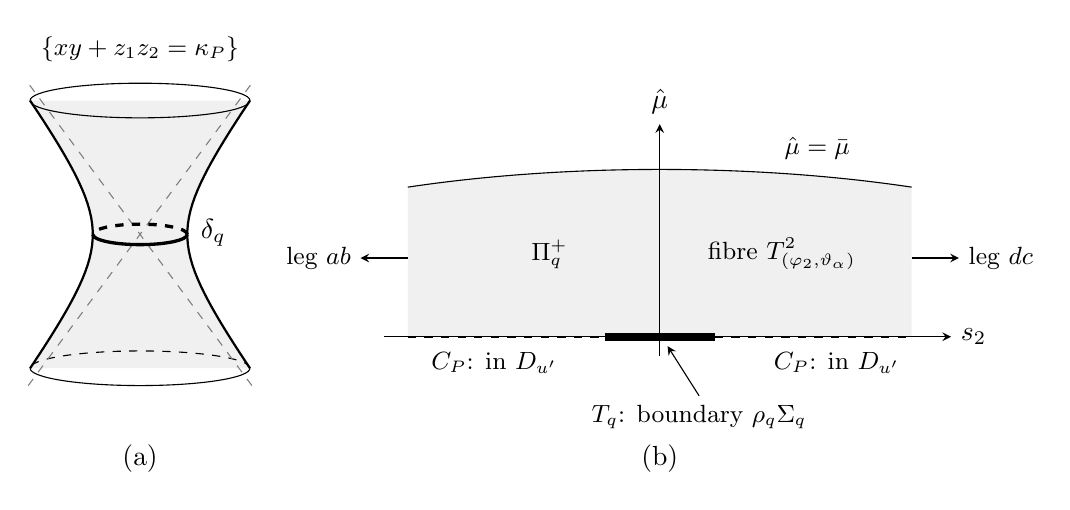
\begin{tikzpicture}[>=stealth]
\begin{scope}
\def\kk{0.6}
\fill[gray!12] plot[domain=-1.7:1.7,samples=40] ({-sqrt(\kk*\kk+0.55*\x*\x)},\x)
  -- plot[domain=1.7:-1.7,samples=40] ({sqrt(\kk*\kk+0.55*\x*\x)},\x) -- cycle;
\draw[thick] plot[domain=-1.7:1.7,samples=40] ({-sqrt(\kk*\kk+0.55*\x*\x)},\x);
\draw[thick] plot[domain=-1.7:1.7,samples=40] ({sqrt(\kk*\kk+0.55*\x*\x)},\x);
\pgfmathsetmacro{\Rr}{sqrt(\kk*\kk+0.55*1.7*1.7)}
\draw (0,1.7) ellipse ({\Rr} and 0.22);
\draw (-\Rr,-1.7) arc (180:360:{\Rr} and 0.22);
\draw[dashed] (\Rr,-1.7) arc (0:180:{\Rr} and 0.22);
\draw[dashed,gray] (-1.42,-1.92) -- (1.42,1.92);
\draw[dashed,gray] (1.42,-1.92) -- (-1.42,1.92);
\draw[very thick] (-\kk,0) arc (180:360:{\kk} and 0.13);
\draw[very thick,dashed] (\kk,0) arc (0:180:{\kk} and 0.13);
\node[right] at (\kk+0.05,0.02) {$\delta_q$};
\node at (0,-2.85) {(a)};
\node[align=center,font=\small] at (0,2.35) {$\{xy+z_1z_2=\kappa_P\}$};
\end{scope}
\begin{scope}[xshift=6.6cm,yshift=-1.3cm]
\fill[gray!12] (-3.2,0) -- (3.2,0) -- (3.2,1.9) .. controls (1.2,2.2) and (-1.2,2.2) .. (-3.2,1.9) -- cycle;
\draw[->] (-3.5,0) -- (3.7,0) node[right] {$s_2$};
\draw[->] (0,-0.25) -- (0,2.7) node[above] {$\hat\mu$};
\draw (3.2,1.9) .. controls (1.2,2.2) and (-1.2,2.2) .. (-3.2,1.9);
\node[font=\small] at (2.0,2.4) {$\hat\mu=\bar\mu$};
\draw[dashed,thick] (-3.2,0) -- (-0.7,0);
\draw[dashed,thick] (0.7,0) -- (3.2,0);
\draw[line width=3pt] (-0.7,0) -- (0.7,0);
\draw[<-] (0.1,-0.12) -- (0.5,-0.75) node[below,font=\small] {$\mathscr T_q$: boundary $\rho_q\Sigma_q$};
\node[below,font=\small] at (-2.1,-0.08) {$\mathscr C_P$: in $D_{u'}$};
\node[below,font=\small] at (2.25,-0.08) {$\mathscr C_P$: in $D_{u'}$};
\draw[->] (-3.2,1.0) -- (-3.8,1.0) node[left,font=\small] {leg $ab$};
\draw[->] (3.2,1.0) -- (3.8,1.0) node[right,font=\small] {leg $dc$};
\node[font=\small] at (-1.4,1.05) {$\Pi^+_q$};
\node[font=\small] at (1.55,1.05) {fibre $T^2_{(\varphi_2,\vartheta_\alpha)}$};
\node at (0,-1.55) {(b)};
\end{scope}
\end{tikzpicture}
\caption{The Morse chart at a node. (a) Schematic real picture of $W^*\cap\mathbb D_P=\{xy+z_1z_2=\kappa_P\}$, two
dimensions lower: in coordinates $\zeta$ with $xy+z_1z_2=\sum_i\zeta_i^2$, the vanishing sphere $\delta_q$ is the waist
$\{\zeta\in\kappa_P^{1/2}\R^4:\sum_i\zeta_i^2=\kappa_P\}$; the dashed lines are the cone of the singular fibre $\kappa_P=0$. (b) The node piece
$\Pi_q^+$ of the $b-a$ passage over the standard half $\{s_1=0,\ \hat\mu\ge0\}$, drawn in the coordinates
$(s_2,\hat\mu)$. Over the interior the fibre is a two-torus (the angle $\varphi_2$ of $\tilde\chi_2$ and the angle
$\vartheta_\alpha$ of $S^1_\alpha$). Over $\hat\mu=0$ the circles $S^1_\alpha$ collapse along $\mathscr C_P$ (dashed), where
$\Pi_q^+$ lies in the divisor $D_{u'}$ and has no boundary; over the thimble $\mathscr T_q$ (thick) they do not, and the
boundary there is the three-sphere $\Sigma_q$, isotopic to $\delta_q$, with multiplicity $\rho_q$
(Lemma~\ref{lem:SI}).}\label{fig:morse}
\end{figure}

\begin{remark}[the sign of $\kappa_P$]\label{rem:kappa}
The window allows both signs of $\eta_P$, hence of $\kappa_P$, and the proof above covers every argument $\phi$ of
$\kappa_P$. The convention of Definition~\ref{def:orient} is also compatible with moving $\kappa_P$ around $0$. In the
family $\{xy+z_1z_2=\kappa\}$, $\kappa=|\kappa|e^{i\phi}$, the sphere $\Sigma^1(\kappa)$ is carried along a path of $\kappa$ by
the complex-linear maps $(x,y,z_1,z_2)\mapsto e^{i\phi/2}(x,y,z_1,z_2)$, which preserve the orientation of the projection
to $(x,z_1)$. A full turn of $\kappa$ acts on $H_3$ of the fibre by the Picard--Lefschetz transformation \cite{Lam81},
which fixes $[\delta]$, because $\langle\delta,\delta\rangle=0$ for the skew intersection form on $H_3$ of a
six-manifold. So the orientations of the $\delta_q$ for different coefficient vectors in $U_\C$ agree under transport.
\end{remark}

\begin{lemma}[change of diagonal]\label{lem:diag}
Replace the labelling $abcd$ of $P$ by $bcda$, which chooses the other diagonal, and keep the order of $u,u'$. Then
$o^{\rm ch}_q$ is unchanged, and the orientation of $\delta_q$ given by Definition~\ref{def:orient} is reversed. Since
$\circv_q$, the coordinate $\lambda_q$ of $K$ and $\rho_q$ change sign as well, $\rho_q\,\delta_q$ and the classes
$\sum_q\lambda_q[\delta_q]$, $\lambda\in K$, do not depend on the choice of diagonals.
\end{lemma}

\begin{proof}
Primes denote the objects of the labelling $a'b'c'd'=bcda$. Then $\mu'_P=\mu_P^{-1}$, $\kappa'_P=e^{\eta_P}-1=-\mu_P\kappa_P$,
$\tilde\chi'_1=\mu_P\tilde\chi_2$, $\tilde\chi'_2=\tilde\chi_1^{-1}$ and $w'_{u'}=-b-w_u$, so $Z$ is unchanged and $Z'$ becomes
$Z'\chi_1^{-1}$; the reference monomial is $b$, so $f'^{(s)}=f^{(s)}/\tilde\chi_1$.

\emph{The chart sign.} Since $\operatorname{val}_c=\operatorname{val}_a+y_1+y_2$, we get $y'_1=y_2$ and $y'_2=-y_1$, and
$\alpha'_q=\alpha_q+\langle\,\cdot\,,b-a\rangle$, which is $\alpha_q+y_1$ up to a constant. The linear map
$(y_1,y_2,\alpha_q)\mapsto(y_2,-y_1,\alpha_q+y_1)$ has determinant $1$, so $o^{\rm ch}_q$ is unchanged.

\emph{The coordinates.} From Definition~\ref{def:morsecoords} and $x'y'+z'_1z'_2-\kappa'_P=f'^{(0)}=f^{(0)}/\tilde\chi_1$ on
$\mathbb D_P$,
\[
x'=y+\mu_P^{1/2}-\mu_P^{-1/2},\qquad y'=\frac{\mu_Px}{\mu_P^{1/2}x-1},\qquad z'_1=c_Zz_1,\qquad z'_2=\frac{z_2}{c_Z\tilde\chi_1},
\]
with a constant $c_Z>0$, the ratio of the two normalisations of $Z$.

\emph{The convention on the thimble.} For $f=xy+z_1z_2-\kappa$ the sphere $\Sigma^1$ bounds the real four-disc
$\{y=e^{i\phi}\bar x,\ z_2=e^{i\phi}\bar z_1,\ |x|^2+|z_1|^2\le|\kappa|\}$, the thimble, which the projection to $(x,z_1)$ maps
onto the ball. So Definition~\ref{def:orient} orients $\delta_q$ as the boundary of the thimble, oriented by $o^{\rm ch}_q$
times the pull-back of the complex orientation of $\C^2_{(x,z_1)}$; for a family of Morse points this orientation is
determined by the tangent space of the thimble at the critical point.

\emph{A deformation.} On $W^*\cap\mathbb D_P$ we have $f^{(0)}=xy+z_1z_2-\kappa_P$. Put $\upsilon:=(1-\mu_P^{1/2}x)^{-1}$, so
that $f'^{(0)}=-\mu_P\,\upsilon f^{(0)}$; on $\mathbb D_P$, $|\mu_P^{1/2}x|\le1/2$, so $\upsilon$ takes values in the disc of
radius $1$ about $1$ without $0$ and has a principal power $\upsilon^s$. For $s\in[0,1]$ the function
$h_s:=\upsilon^sf^{(0)}$ has zero set $W^*\cap\mathbb D_P$. Its critical points satisfy $x=z_1=z_2=0$ (from the derivatives in
$y,z_2,z_1$, since $\upsilon\ne0$) and then $y=s\mu_P^{1/2}\kappa_P$: there is exactly one, $q_s$, with value $-\kappa_P$.
Its Hessian is that of $f^{(0)}$ plus $c_s\,dx^2$, $c_s=s(s-1)\mu_P\kappa_P$; since the matrix $\bigl(\begin{smallmatrix}c&1\\
1&0\end{smallmatrix}\bigr)$ is invertible for every $c$, $q_s$ is nondegenerate. The tangent space of its thimble for the
straight path from $-\kappa_P$ to $0$ is
\[
T_s=\bigl\{v:\ v_y=e^{i\phi}\bar v_x-\tfrac{c_s}2v_x,\ v_{z_2}=e^{i\phi}\bar v_{z_1}\bigr\},
\]
on which the Hessian form is $2e^{i\phi}(|v_x|^2+|v_{z_1}|^2)$; it is a graph over the $(x,z_1)$-plane for every $s$. So the
vanishing spheres of $q_s$ form a continuous family in $W^*\cap\mathbb D_P$, and orienting each as the boundary of its
thimble with the orientation pulled back from $\C^2_{(x,z_1)}$ is continuous in $s$. At $s=0$ this is the orientation of
Definition~\ref{def:orient} for $abcd$ (up to the common factor $o^{\rm ch}_q$). At $s=1$, $h_1=-\mu_P^{-1}f'^{(0)}$ has the
same level sets as $f'^{(0)}$ along the straight paths, so its vanishing sphere is, up to isotopy, the one of the
labelling $bcda$, whose convention pulls back the orientation of $\C^2_{(x',z'_1)}$. The sphere of that convention is
linear in the primed coordinates, and the tangent plane $T'$ of its thimble at $q_1$ need not be $T_1$. At $q_1$, where
$c_1=0$, $\operatorname{Hess}f'^{(0)}=-\mu_P\operatorname{Hess}h_1=-\mu_P\operatorname{Hess}f^{(0)}$, and the path of
$f'^{(0)}$ runs from its critical value $-\kappa'_P$ towards $0$, in the direction of $\kappa'_P=-\mu_P\kappa_P$; so
$\bar\kappa'_P\operatorname{Hess}f'^{(0)}=|\mu_P|^2\,\bar\kappa_P\operatorname{Hess}f^{(0)}$.
Hence $T_1$ and $T'$ are both real four-planes on which $e^{-i\phi}\operatorname{Hess}f^{(0)}$ is real and positive
definite; in particular both are maximal positive planes of the real quadratic form
$\operatorname{Re}(e^{-i\phi}\operatorname{Hess}f^{(0)})$ at $q_1$. After a complex-linear change of coordinates in which
$e^{-i\phi}\operatorname{Hess}f^{(0)}$ becomes $\sum_i\zeta_i^2$, the planes of this kind are the images of $\R^4$ under
$O(4,\C)$, so they form a family $O(4,\C)/O(4)$, which is connected since $O(4)$ meets both components of $O(4,\C)$; the linear thimbles they contain have their boundary spheres
in one level set of the quadratic part, and these spheres move by isotopy along the family. Both thimbles at $q_1$ are
such linear thimbles in one chart. Let $\mathbf w':=(x',y',z'_1,z'_2)$, $A:=d\mathbf w'(q_1)$ and $\mathbf w:=A^{-1}\mathbf w'$.
Since $\mathbf w'(q_1)=0$ and $Q'\circ A=-\mu_PQ$ for the quadratic parts $Q$, $Q'$ of $h_1$ and $f'^{(0)}$ at $q_1$, we have
$h_1=-\mu_P^{-1}f'^{(0)}=-\mu_P^{-1}(Q'(A\mathbf w)-\kappa'_P)=Q(\mathbf w)-\kappa_P$ on $\mathbb D_P$, so $\mathbf w$ are
holomorphic Morse coordinates of $h_1$ at $q_1$ tangent to the identity. In them the thimble of $q_1$ is the linear thimble
with tangent plane $T_1$, and the thimble of the primed convention is the linear thimble with tangent plane
$T'=A^{-1}T'_{\rm lin}$, where $T'_{\rm lin}$ is its tangent plane in the coordinates $\mathbf w'$. So the orientations of $\delta_q$ induced
from oriented thimbles are carried along this family of planes by continuity. On each of them the projections to $(v_x,v_{z_1})$ and to $(v_{x'},v_{z'_1})$, that is to
$(v_y,v_{z_1})$ up to a complex-linear change, are isomorphisms, because a vector with $v_x=v_{z_1}=0$, or with
$v_y=v_{z_1}=0$, is isotropic. So the sign relating the two pulled-back orientations is constant on the family, and it
suffices to compute it on $T_1$. On $T_1$ (where $c_1=0$) the differential of
$(x,z_1)\mapsto(x',z'_1)$ is $(v_x,v_{z_1})\mapsto(e^{i\phi}\bar v_x,c_Zv_{z_1})$, which reverses orientation. So the two
conventions orient $\delta_q$ oppositely.
\end{proof}
